\documentclass[9pt,twocolumn,a4paper]{extarticle}

% ============================================================================
% PACKAGES
% ============================================================================

% Core formatting
\usepackage[utf8]{inputenc}
\usepackage[T1]{fontenc}
\usepackage{lmodern}
\usepackage[margin=0.75in,columnsep=0.28in]{geometry}
\usepackage{microtype}
\usepackage{xurl}

% Compact heading spacing: the class defaults open a gap at every section boundary that reads
% as a break. Sections run on, separated by the heading itself.
\usepackage{titlesec}
\usepackage{dblfloatfix}
\usepackage{cuted}
\usepackage{subcaption}
\titlespacing*{\section}{0pt}{1.4ex plus 0.4ex minus 0.2ex}{0.8ex plus 0.2ex}
\titlespacing*{\subsection}{0pt}{1.1ex plus 0.3ex minus 0.2ex}{0.6ex plus 0.2ex}
% Floats fill pages instead of pushing text to the next column and leaving the gap behind.
\renewcommand{\topfraction}{0.92}
\renewcommand{\dbltopfraction}{0.92}
\renewcommand{\textfraction}{0.06}
\renewcommand{\floatpagefraction}{0.85}
\renewcommand{\dblfloatpagefraction}{0.85}

% Mathematics
\usepackage{amsmath,amssymb,amsthm}
\usepackage{algorithm}
\usepackage{algpseudocode}

% Graphics and figures
\usepackage{graphicx}
\usepackage{tikz}
\usepackage{pgfplots}
\pgfplotsset{compat=1.18}
\usetikzlibrary{shapes,arrows,positioning,calc}

% Tables
\usepackage{booktabs}
\usepackage[section]{placeins}
\usepackage{array}

% Code listings
\usepackage{listings}
\lstset{
    basicstyle=\small\ttfamily,
    keywordstyle=\color{blue}\bfseries,
    commentstyle=\color{gray}\itshape,
    stringstyle=\color{red},
    numbers=left,
    numberstyle=\tiny\color{gray},
    breaklines=true,
    frame=single,
    captionpos=b
}

% Colors
\usepackage{xcolor}
\definecolor{wolfram}{RGB}{221,51,51}

% Hyperlinks
\usepackage[colorlinks=true,linkcolor=blue,citecolor=blue,urlcolor=blue]{hyperref}

% Bibliography
\usepackage[numbers,sort&compress]{natbib}

% Theorem environments
\newtheorem{theorem}{Theorem}[section]
\newtheorem{lemma}[theorem]{Lemma}
\newtheorem{proposition}[theorem]{Proposition}
\newtheorem{corollary}[theorem]{Corollary}
\newtheorem{definition}[theorem]{Definition}
\newtheorem{remark}[theorem]{Remark}

% Custom commands
\newcommand{\BigO}{\mathcal{O}}
\newcommand{\hypergraph}{\mathcal{H}}
\newcommand{\state}{\mathcal{S}}
\newcommand{\event}{\mathcal{E}}
\newcommand{\rewriterule}{\mathcal{R}}
\newcommand{\match}{\mathcal{M}}
\newcommand{\hash}{\textup{\textsc{Hash}}}
\newcommand{\canon}{\textup{\textsc{Canon}}}



% ============================================================================
% DOCUMENT
% ============================================================================
% GENERATED by tools/dev/paper_tables.py -- do not edit.
% commit e6f26a9d | measured on Intel(R) Core(TM) i9-14900K, 31 GB RAM, Linux 5.15.167.4-microsoft-standard-WSL2 | load at start 0.19/0.23 (1m/15m) | source: the generators in this file

\newcommand{\AuthorityDeepSeconds}{428}
\newcommand{\CoreDeepMs}{8.5}
\newcommand{\PacletDeepSeconds}{0.14}
\newcommand{\PacletOverheadDeep}{16}
\newcommand{\PacletVsAuthorityDeep}{3081}
\newcommand{\SpeedupAtHighDepth}{50{,}384}
\newcommand{\SpeedupAtLowDepth}{1{,}696}
\newcommand{\SpeedupHighDepth}{7}
\newcommand{\SpeedupLowDepth}{4}
% carried forward from the previous generation of this file: their
% measurement did not run in this invocation, and the prose cites them.
\newcommand{\GpuDeepestDepth}{7}
\newcommand{\GpuSpeedupAtDeepest}{2.3}
\newcommand{\MaxHostSpeedup}{3.6}
\newcommand{\MaxHostSpeedupThreads}{32}
  % generated: macros the prose cites, so a regenerated table moves them
% GENERATED by tools/dev/paper_tables.py -- do not edit.
% commit 769b12ba | Intel(R) Core(TM) i9-14900K, 20 GB RAM, Linux 5.15.167.4-microsoft-standard-WSL2 | source: the generators in this file

\newcommand{\EffAtEight}{0.79}
\newcommand{\EffAtSixteen}{0.51}
\newcommand{\SaturationBlocks}{4}
\newcommand{\SysTimeGrowth}{16}
\newcommand{\ThreadSweepFactor}{32}
\newcommand{\UserTimeGrowth}{1.7}

% GENERATED by tools/dev/paper_tables.py -- do not edit.
% commit 61c409ca | measured on AMD EPYC 9174F 16-Core Processor, NVIDIA RTX 4090 | source: tools/bench_gpu_evolve.cpp (mode 0)
\newcommand{\PersistentSpeedupFour}{16.5}
\newcommand{\PersistentSpeedupFive}{13.3}
\newcommand{\PersistentSpeedupSix}{5.4}
\newcommand{\PersistentSpeedupSeven}{4.2}
\newcommand{\PersistentSpeedupEight}{0.96}
\newcommand{\PersistentSpeedupNine}{0.97}
\newcommand{\PersistentEvolveConstLo}{49}
\newcommand{\PersistentEvolveConstHi}{56}
\newcommand{\PersistentStatesLo}{53}
\newcommand{\PersistentStatesHi}{3{,}867}
\newcommand{\PersistentTieDepthWord}{eight}
\newcommand{\PersistentStatesTie}{262{,}144}

% GENERATED by tools/dev/paper_tables.py -- do not edit.
% commit 61c409ca | measured on AMD EPYC 9174F 16-Core Processor | source: callgrind_annotate over the attrib phase
\newcommand{\InstrFlatCoverage}{99.0}


\begin{document}

% ----------------------------------------------------------------------------
% TITLE
% ----------------------------------------------------------------------------

\title{\textbf{Rewriting the Universe}\\[0.4em]
{\normalsize\normalfont High-Performance Hypergraph Rewriting for the Wolfram Physics Project}}

\author{
    Richard Assar\\
    \textit{Wolfram Institute}\\
    \texttt{rassar@wolframinstitute.org}
}

\date{\today}

\maketitle

% ----------------------------------------------------------------------------
% ABSTRACT
% ----------------------------------------------------------------------------

\begin{abstract}
The Wolfram Physics Project models fundamental physics by hypergraph rewriting. Multiway
evolution applies every applicable rewrite to every reachable state and records the states up to
isomorphism, the events between them, and the causal and branchial relations over the events.
For rules that add edges, the number of states grows super-exponentially with depth. We present a
multiway hypergraph rewriting engine for CPU and GPU. Every state is identified by the hash of an exact
McKay-style individualization--refinement canonical form, computed by one implementation shared
by the CPU and the GPU's resident evolution kernel. The engine is lock-free, runs without phases
or passes, maintains the causal and branchial relations and the causal graph's transitive
reduction as events are created, and returns the same output at every thread count. Quotient
exploration expands one state per isomorphism class and reconstructs the raw events and relations
exactly. The concurrent data structures and protocols are model-checked under the RC11 memory
model and its GPU-scoped extension, and four protocols are also model-checked under TLA+ for any
number of workers.
Against the \texttt{Wolfram/\allowbreak Multicomputation} paclet's \texttt{MultiwaySystem},
with identical state and causal-edge counts at every depth, the engine's C++ core is
$\SpeedupAtLowDepth\times$ faster at depth \SpeedupLowDepth{} and $\SpeedupAtHighDepth\times$
faster at depth \SpeedupHighDepth{} on an Intel i9-14900K. The engine is available as a C++/CUDA
library and as a Wolfram Language paclet.

\vspace{1em}
\noindent\parbox{\linewidth}{\textbf{Keywords:} hypergraph rewriting, graph canonicalization,
multiway systems, GPU computing, Wolfram Physics Project}
\end{abstract}

% ----------------------------------------------------------------------------
% INTRODUCTION
% ----------------------------------------------------------------------------

\section{Introduction}
\label{sec:introduction}

The Wolfram Physics Project~\cite{wolfram2020project} models the universe as an abstract rewrite system, in which physics is given by the causal structure of the rewrites rather than by the data being rewritten. The states are hypergraphs, which have no built-in notion of space: distance is path length through the edges. Rewriting produces three structures: the multiway evolution graph of all reachable states and the events between them; the causal graph, of dependencies between events; and the branchial graph, of pairs of events that consume a common edge of the same state.

Exhaustive multiway evolution is expensive. Each step multiplies the number of histories by the frontier's match count, and a rule that adds edges gives each state more matches than its parent, so the count grows super-exponentially: on the canonical Wolfram rule the ratio between consecutive depths rises from $1.7$ at depth two to $11.7$ at depth seven. Every step matches the rule against each new state, canonicalizes each new state to detect isomorphic duplicates, and records events and their causal and branchial relations. The existing Wolfram Language implementation takes $\AuthorityDeepSeconds$\,s to reach depth \SpeedupHighDepth{} of the corpus's \texttt{wolfram-2to4} rule; this engine takes $\CoreDeepMs$\,ms for the same evolution (Section~\ref{sec:benchmarks}).

The engine provides:

\begin{enumerate}
    \item \textbf{Exact canonicalization:} Every state is canonicalized by McKay-style individualization--refinement (IR)~\cite{mckay2014practical}, and the canonical hash is the deduplication key, so two states are identified if and only if they are isomorphic. Proposition~\ref{prop:wlceiling} bounds the saving from any cheaper filter in front of IR by the ratio of canonical classes to raw states, which falls toward zero with depth.

    \item \textbf{Lock-free concurrency:} The engine holds no lock. Its hash maps, segmented arrays, lists and work-stealing deques are non-blocking, and an idle worker waits on an atomic counter through \texttt{futex}~\cite{franke2002fuss} on Linux, \texttt{WaitOnAddress} on Windows or \texttt{os\_sync\_wait\_on\_address} on macOS, using no cycles until new work arrives.

    \item \textbf{GPU acceleration:} A CUDA kernel that stays resident for the whole evolution runs matching, rewriting and canonicalization, so no step returns to the host. It is faster than the CPU when the rule set gives it enough independent work (Section~\ref{sec:benchmarks}).

    \item \textbf{Configurable equivalence:} State and event identity are chosen independently. State identity is \textsc{None}, \textsc{Automatic} (a content hash) or \textsc{Full} (exact IR); event identity is built from a small set of signature keys.

    \item \textbf{Exploration strategies:} Quotient exploration (Section~\ref{sec:quotient}) expands one state per isomorphism class and still reconstructs every raw event; sampling with per-rule rates and a per-state match cap (Section~\ref{sec:sampling}) reaches depths where exhaustive evolution cannot; and the causal graph's transitive reduction (Section~\ref{sec:tr}) is maintained as edges are added.

    \item \textbf{Determinism:} The state set, event set and causal and branchial relations depend only on the inputs, not on the thread count or the scheduling order (Section~\ref{sec:determinism}).
\end{enumerate}

Section~\ref{sec:background} reviews hypergraph rewriting and related work; Section~\ref{sec:canonicalization} describes canonicalization; Section~\ref{sec:pattern-matching} the pattern matcher; Section~\ref{sec:architecture} the system architecture; Section~\ref{sec:gpu} the GPU implementation; Section~\ref{sec:benchmarks} the evaluation; and Section~\ref{sec:verification} the verification of the concurrent code. Section~\ref{sec:conclusion} concludes.

% ----------------------------------------------------------------------------
% BACKGROUND
% ----------------------------------------------------------------------------


\section{Background and Related Work}
\label{sec:background}

This section defines rules, matches, the multiway evolution graph and the causal and branchial
relations, and reviews related systems.

\subsection{Hypergraph Rewriting Systems}

A \emph{hypergraph} $\hypergraph = (V, E)$ consists of a vertex set $V$ and a set of hyperedges $E$, where each hyperedge $e \in E$ is an ordered tuple of vertices $(v_1, v_2, \ldots, v_k)$ with $v_i \in V$. The Wolfram Physics Project uses hypergraphs because distance in them is path length, which gives rewriting a notion of locality without fixing a space in advance, as strings and cellular automata do.

\begin{definition}[Rewriting Rule]
A rewriting rule $\rewriterule = (L, R)$ consists of a left-hand side pattern $L$ and right-hand side replacement $R$, both hypergraphs. A \emph{match} of $L$ in $\hypergraph$ is an injective mapping $\phi: V_L \to V_\hypergraph$ such that the image of each hyperedge in $L$ appears in $\hypergraph$.
\end{definition}

Rules are applied in the single-pushout form: the matched image is deleted and the replacement glued in, without the gluing conditions of the double-pushout construction~\cite{ehrig2006fundamentals,rozenberg1997handbook,plump2009graph}. Applying rule $\rewriterule$ at match $\phi$ produces a new hypergraph $\hypergraph'$ by:
\begin{enumerate}
    \item Removing all hyperedges in $\phi(L)$ from $\hypergraph$
    \item Adding hyperedges from $R$, extending $\phi$ to map new vertices in $R$ to fresh vertices
\end{enumerate}

\subsection{Multiway Evolution}

\emph{Multiway evolution} applies every applicable rule at every match of every state, producing a directed graph of states connected by events. Figure~\ref{fig:worked-example} shows two steps of a small rule in full: the raw states, the canonical states they reduce to, the events and the causal edges.

\begin{definition}[Evolution Graph]
Given initial state $\state_0$ and rule set $\{\rewriterule_i\}$, the evolution graph $G = (\state, \event)$ contains:
\begin{itemize}
    \item States $\state$: all hypergraphs reachable from $\state_0$
    \item Events $\event$: transitions $(s, s', r, \phi)$ where state $s$ rewrites to $s'$ via rule $r$ at match $\phi$
\end{itemize}
\end{definition}

\begin{figure*}[htbp]
\centering
% GENERATED by tools/dev/object_figure.wls -- do not edit.
% commit 316a7384 | measured on fly_desktop2 | raw states 4, canonical 3, events 3, causal 2, branchial 0 | source: tools/dev/object_figure.wls
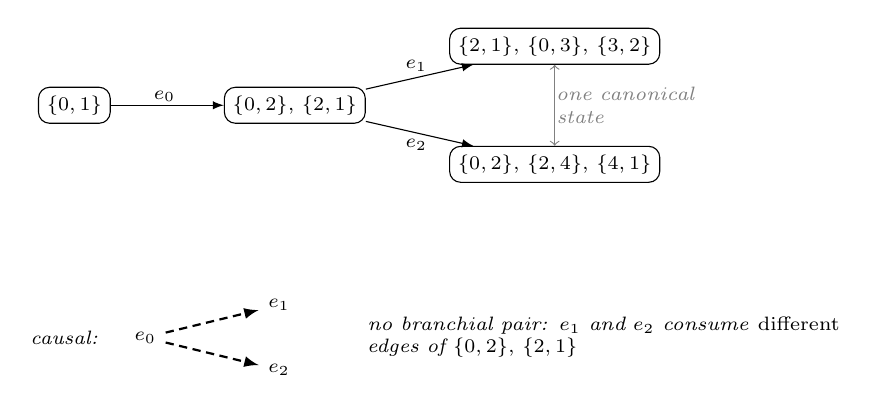
\begin{tikzpicture}[
    st/.style={rectangle, draw, rounded corners, inner sep=3pt, font=\scriptsize},
    ev/.style={->, >=latex, thin},
    cau/.style={->, >=latex, thick, densely dashed},
    lbl/.style={font=\scriptsize\itshape, inner sep=1pt}
]
\node[st] (s0) at (0,0.0) {$\{0,1\}$};
\node[st] (s1) at (2.8,0.0) {$\{0,2\},\,\{2,1\}$};
\node[st] (s2) at (6.1,0.75) {$\{2,1\},\,\{0,3\},\,\{3,2\}$};
\node[st] (s3) at (6.1,-0.75) {$\{0,2\},\,\{2,4\},\,\{4,1\}$};
\draw[ev] (s0) -- node[lbl, above left, pos=0.6]{$e_{0}$} (s1);
\draw[ev] (s1) -- node[lbl, above left, pos=0.6]{$e_{1}$} (s2);
\draw[ev] (s1) -- node[lbl, below left, pos=0.6]{$e_{2}$} (s3);
\draw[<->, gray, thin] (s2) -- node[lbl, right, text width=2.1cm]{one canonical state} (s3);
\node[lbl, anchor=west] at (-0.6,-2.95) {causal:};
\node[font=\scriptsize] (c0) at (0.9,-2.95) {$e_{0}$};
\node[font=\scriptsize] (c1) at (2.6,-2.5375) {$e_{1}$};
\node[font=\scriptsize] (c2) at (2.6,-3.3625) {$e_{2}$};
\draw[cau] (c0) -- (c2);
\draw[cau] (c0) -- (c1);
\node[lbl, anchor=west, text width=6.2cm] at (3.7,-2.95) {no branchial pair: $e_{1}$ and $e_{2}$ consume \emph{different} edges of $\{0,2\},\,\{2,1\}$};
\end{tikzpicture}

\caption{Two steps of $\{x,y\} \rightarrow \{x,z\},\{z,y\}$ from a single edge, as the engine
reports them. Four raw states reduce to three canonical states, because the two depth-2 results
are isomorphic. Both causal edges come from $e_0$, because each depth-2 event consumes one of the
two edges $e_0$ produced. The branchial relation is empty: $e_1$ and $e_2$ start from the same
state but consume different edges. Every element is taken from the engine's output.}
\label{fig:worked-example}
\end{figure*}

The \emph{causal graph} has an edge from event $p$ to event $c$ when $c$ consumes an edge that $p$ produced. The \emph{branchial graph} has an edge between two events that consume a common edge of the same state; it records where the evolution branches, which the Wolfram Physics Project relates to quantum superposition~\cite{wolfram2020project}.

\subsection{The Graph Isomorphism Problem}

Deduplicating states requires deciding whether two hypergraphs are isomorphic, that is, equal up to a relabeling of vertices. Graph isomorphism is in NP and is not known to be NP-complete or to be in P~\cite{kobler2012graph}; the best known algorithm is quasipolynomial~\cite{babai2016quasipolynomial}. This engine computes an exact canonical form for every state, so its canonical hash is equal for two states if and only if they are isomorphic (Section~\ref{sec:canonicalization}).

\subsection{Related Work}

\textbf{Graph canonicalization:} The nauty/Traces line of work~\cite{mckay2014practical} established individualization--refinement (IR) as the standard exact method for graph canonicalization. It is exponential in the worst case and fast on typical instances, and it is the canonicalizer this engine uses. Weisfeiler--Leman color refinement~\cite{weisfeiler1968reduction,shervashidze2011weisfeiler} runs in polynomial time but gives the same value to some non-isomorphic graphs, so it cannot serve as an exact identity.

\textbf{Hypergraph rewriting implementations:} SetReplace~\cite{setreplace} is the implementation
most closely associated with the Wolfram Physics Project, and it computes a different object. Its
multiway construction is a token--event graph over one growing pool of tokens: its vertices are
tokens and events rather than states, a token consumed by one event remains available to others,
and no state identity is computed. Its only isomorphism test during evolution is an optional
deduplication of events with the same input tokens and isomorphic outputs. This engine enumerates
the states graph under exact isomorphism, which requires canonicalizing every state as it is
produced (Section~\ref{sec:canonicalization}), so canonicalization rather than matching dominates
its cost. A wall-time comparison between the two would compare different computations.
Section~\ref{sec:benchmarks} therefore compares against two implementations of the same object: the
\texttt{Wolfram/\allowbreak Multicomputation} paclet's
\texttt{MultiwaySystem}~\citep{wolframmulticomputation}\footnote{Distributed through the Wolfram
Paclet Repository,
\url{https://resources.wolframcloud.com/PacletRepository/resources/Wolfram/Multicomputation/}.
Every comparison uses version 0.1.8, the latest published release (23 November 2024; checked 31
August 2026).}, all of whose properties return Wolfram \texttt{Graph} objects, so its time
includes building them; and this project's \emph{reference implementation}, a direct transcription
of the definition that returns data rather than graphs and serves as the correctness oracle
throughout. \emph{Reference implementation} always means the latter.

\textbf{Subgraph matching on hypergraphs:} HGMatch~\cite{yang2023hgmatch} matches one hyperedge at a time rather than one vertex at a time, seeding a join from one pattern hyperedge and extending it by one hyperedge per step; it restricts candidates by a label-derived signature, and runs as a dataflow on a work-stealing task scheduler. This engine's matcher uses all three. Hyperedges here are unlabelled, so the signature is the edge's vertex-repetition pattern (Definition~\ref{def:signature}). When an expansion has a variable already bound, its candidates come from the vertex index rather than the signature bucket; on the device this reduced match-kernel time on one workload from 944\,ms to 4\,ms.

\textbf{GPU graph algorithms:} GPUs have been applied to subgraph matching~\cite{tran2015fast}, graph mining~\cite{chen2021pangolin} and general graph algorithms~\cite{wang2016gunrock}. This engine's match kernel follows the warp-centric organization of G2Miner~\cite{chen2022g2miner}: one block per (state, rule) pair, its threads dividing the seed candidates and each running its own depth-first search. Unlike these systems, the kernel stays resident across evolution steps, because each step's output states are the next step's inputs.

\textbf{Dynamic graph algorithms:} The causal graph's transitive reduction is maintained as edges are added. Goranci et al.~\cite{goranci2025dynamic} give fully dynamic transitive-reduction algorithms under insertions and deletions in $\BigO(m + n\log n)$ amortized time. This engine's case has insertions only, arriving in topological order, from concurrent workers, and the retained edge set must not depend on the schedule (Section~\ref{sec:tr}).

\textbf{Term rewriting:} Term rewriting theory~\cite{baader1998term} treats confluence and termination for tree-structured terms, and fast implementations~\cite{van2019fastest} optimize similar pattern matching. In hypergraph rewriting the objects are graphs, so matching is subgraph matching rather than tree matching, and states are compared up to isomorphism rather than syntactic equality.

% ----------------------------------------------------------------------------
% CANONICALIZATION
% ----------------------------------------------------------------------------


\section{State and Event Identity}
\label{sec:canonicalization}

Deduplication decides how large the explored set is: without it, every path to a state adds a separate vertex, and the number of paths grows super-exponentially when rewrites add edges. Two states are the same node when their hypergraphs are isomorphic, with vertex relabeling allowed and within-edge order and edge multiplicity preserved. The exact mode computes an individualization--refinement (IR) canonical form for every state and deduplicates by a 64-bit hash of that form, which two isomorphic states always share; two non-isomorphic states share it only through a hash collision, which the engine does not check for.

\subsection{Individualization--Refinement}
\label{sec:ir}

The canonical form is computed by McKay-style individualization--refinement~\cite{mckay2014practical}, the family of algorithms behind nauty and Traces. IR produces a canonical labeling, together with automorphism generators and vertex and edge orbits, such that two hypergraphs receive the same canonical form if and only if they are isomorphic.

\begin{definition}[Canonical Form]
A canonicalization $\canon$ maps each hypergraph to a labeled representative such that $\canon(\hypergraph_1) = \canon(\hypergraph_2)$ iff $\hypergraph_1 \cong \hypergraph_2$.
\end{definition}

IR refines a vertex coloring until it is stable. If a cell with more than one vertex remains, it \emph{individualizes} one of its vertices (gives it a unique color) and recurses, which produces a search tree of refinements. Automorphisms found during the search prune symmetric branches, and the lexicographically extremal leaf defines the canonical labeling.

\begin{remark}[Complexity]
Like nauty, IR is exponential in the worst case and polynomial in the state size on states without large automorphism groups. The worst case occurs on highly symmetric states, where the exact mode's cost is concentrated. Proposition~\ref{prop:wlceiling} bounds what a cheaper filter in front of IR can save.
\end{remark}

The automorphism generators and edge orbits from IR are used again for event canonicalization and for the exact reconstruction of causal and branchial multiplicities.

\paragraph{Search bounds.} The search has two bounds: the individualization depth and the number of automorphism generators recorded. Exceeding either is reported, and the engine raises the bound and runs the search again. The two fail differently. Reaching the depth bound before the coloring is discrete produces no canonical form, so the failure is visible. A full generator table still produces a correct canonical hash, but the orbits, which are built by fusing edges over the recorded generators, come out too fine. The quotient reconstruction identifies instances by these orbits (Section~\ref{sec:quotient}), so a truncated generator table would give a wrong result with no error. The generator bound is therefore raised on overflow in the same way as the depth bound. Raising the generator bound cannot fix a depth failure, so escalation stops at the first depth failure.

\paragraph{Symmetric states.} When a state has nontrivial automorphisms, IR selects one of several equivalent labelings by a tie-break within cells, and the tie-break depends on the order in which the state's vertices are numbered. Two numbering conventions give the same canonical hash but can assign different ranks to the same edge. Edge ranks identify consumed and produced edges across a rewrite, so one numbering convention is shared by every caller. On the equivalence probe's 4063-state corpus, encounter-order numbering and sorted-unique numbering assign different ranks on 103 states, all with nontrivial automorphisms.

\subsection{A Ceiling on Pre-Filters}
\label{sec:wl}

A sound invariant cheaper than IR, such as Weisfeiler--Leman color refinement~\cite{weisfeiler1968reduction,shervashidze2011weisfeiler}, could filter states before canonicalization: hash every state cheaply and run IR only when the cheap hash repeats. Proposition~\ref{prop:wlceiling} bounds the saving.

\begin{proposition}[Ceiling on a pre-filter]
\label{prop:wlceiling}
Let a run produce $R$ raw states falling into $C$ isomorphism classes, and let $f$ be a sound isomorphism invariant: isomorphic states receive equal $f$-values. Consider deduplication that computes $f$ on each raw state, and invokes IR only when the value has been seen before. Then the number of IR invocations is at least $R - C$, so the fraction of IR calls avoided is at most $C/R$, and one $f$-pass is paid on all $R$ states.
\end{proposition}

\begin{proof}
Soundness means states in one class share an $f$-value, so the number of distinct values is at most $C$. A state whose value is already present cannot be resolved by $f$: equal values are consistent both with isomorphism and with an $f$-collision, so IR is invoked. At most one state per distinct value finds its value absent, hence at most $C$ states skip IR and at least $R - C$ invoke IR.
\end{proof}

$C/R$ depends on the rule and the depth. Table~\ref{tab:crratio} and Figure~\ref{fig:crratio} give it for each corpus workload at two depths.

\begin{table}[htbp]
\centering
\caption{\textbf{Canonical classes as a fraction of raw states, per corpus workload.} $C/R$ is
the upper bound of Proposition~\ref{prop:wlceiling} on the fraction of IR calls a pre-filter can
skip. The event count is given beside it because a ratio from a small run is weaker evidence than
the same ratio from a large one.}
\label{tab:crratio}
% GENERATED by tools/dev/paper_tables.py -- do not edit.
% commit 1d5bc1c9 | Intel(R) Core(TM) i9-14900K, 20 GB RAM, Linux 5.15.167.4-microsoft-standard-WSL2 | source: tools/cost_matrix.cpp
\resizebox{\ifdim\width>\linewidth\linewidth\else\width\fi}{!}{%
\begin{tabular}{llrrr}
\toprule
Case & Rule type & Events & $C/R$ & $C/R$ at lower depth \\
\midrule
\texttt{cycle4-automorphic} & automorphism & 68{,}184 & 0\% & 12\% \\
\texttt{star4-automorphic} & automorphism & 68{,}184 & 0.3\% & 20\% \\
\texttt{disconnected-lhs} & disconnected & 126 & 0.8\% & 14.3\% \\
\texttt{binary-growth} & productive/arity2 & 873 & 4.1\% & 75\% \\
\texttt{multi-rule} & multi-rule & 237 & 15.1\% & 83.3\% \\
\texttt{triangle} & productive/mixed-conn & 124 & 28.8\% & 60\% \\
\texttt{arity3-growth} & arity3 & 153 & 42.2\% & 100\% \\
\texttt{self-loop} & self-loop/arity2 & 1 & 100\% & 100\% \\
\bottomrule
\end{tabular}
}

\end{table}

% GENERATED by tools/dev/paper_tables.py -- do not edit.
% commit 9fb1039 | measured on AMD EPYC 9174F 16-Core Processor, 503 GB RAM, Linux 6.8.0-138-generic | load at start 3.09/2.50 (1m/15m) | source: tools/cost_matrix.cpp

\pgfplotsset{crsymbolic/.style={symbolic x coords={cycle4,star4,disconn,binary,multi,triangle,arity3,self-loop}}}

\begin{figure}[tb]
\centering
\resizebox{\linewidth}{!}{%
\begin{tikzpicture}
\begin{axis}[
    width=\linewidth, height=4.8cm,
    ybar, bar width=2.2pt,
    ylabel={$C/R$ (\%)}, ymin=0, ymax=105,
    crsymbolic,
    xtick=data, x tick label style={font=\scriptsize, rotate=20, anchor=east},
    grid=major, grid style={gray!25},
    legend style={font=\scriptsize, at={(0.02,0.97)}, anchor=north west, draw=none, fill=none},
    label style={font=\small}, tick label style={font=\scriptsize},
]
% GENERATED by tools/dev/paper_tables.py -- do not edit.
% commit 4f4af3d | measured on AMD EPYC 9174F 16-Core Processor, 503 GB RAM, Linux 6.8.0-138-generic | load at start 1.34/1.00 (1m/15m) | source: tools/cost_matrix.cpp

\addplot[fill=gray!55, draw=black] coordinates {(cycle4,12)(star4,20)(disconn,14.3)(binary,75)(multi,83.3)(triangle,60)(arity3,100)(self-loop,100)};
\addlegendentry{lower depth}
\addplot[fill=white, draw=black] coordinates {(cycle4,0)(star4,0.3)(disconn,0.8)(binary,4.1)(multi,15.1)(triangle,28.8)(arity3,42.2)(self-loop,100)};
\addlegendentry{higher depth}

\end{axis}
\end{tikzpicture}}
\caption{$C/R$ for each corpus workload at two depths: the upper bound of
Proposition~\ref{prop:wlceiling} on the fraction of IR calls a pre-filter can skip. It falls with
depth on every workload that keeps rewriting. \texttt{self-loop} reaches a fixed point after one
event and stays at $100\%$. Values as in Table~\ref{tab:crratio}.}
\label{fig:crratio}
\end{figure}

\noindent On every rule that keeps rewriting, $C/R$ falls with depth, because multiway evolution reaches the same state along many histories and each repeat is a repeated filter value that IR must still resolve. The ratio stays high only on workloads that reach a fixed point within one or two steps, such as \texttt{self-loop} ($C/R = 100\%$ over two raw states and one event), and those have little canonicalization work to save.

The one exact shortcut, reusing a canonical form when two raw states have identical edge tuples, never applies: every rewrite assigns fresh vertex identifiers, so on \texttt{wpp} the number of distinct state contents equals the number of raw states at depths six and seven ($3{,}867$ and $45{,}317$).

Quotient exploration and the event identities of Section~\ref{sec:event-canon} need automorphism data, and both take the edge orbits from the same IR pass.

\subsection{State Canonicalization Modes}

The engine's \emph{state canonicalization mode} sets how states are identified. \textsc{None} keeps every raw state distinct. \textsc{Automatic} deduplicates by a hash of the edge tuples as given, which is not an isomorphism invariant: it identifies two states only when their edge tuples are equal, so isomorphic states with different vertex labels stay distinct. \textsc{Full} is the exact mode: the IR canonical hash of every state is the deduplication key.

\subsection{Event Identity}
\label{sec:event-canon}

Events can be identified at three granularities:

\begin{description}
\item[ByEndpointStates:] Two applications are the same event when they run between the same pair of canonical states. $\BigO(1)$ signature computation.

\item[ByConsumedProducedEdges:] The signature additionally includes the canonical ranks of the edges the application consumed and produced. $\BigO(E)$ signature computation.

\item[DistinctApplications:] No signature is computed and every application is its own event. This is the identity the raw causal graph is defined over.
\end{description}

Each refines the one before, so the event count is non-decreasing in that order;
Table~\ref{tab:event-canon} gives it per workload. \textsc{ByConsumedProducedEdges} needs the
correspondence between the edges of isomorphic states, which is the per-edge canonical rank from
the same IR pass as the state's hash.

\paragraph{Independence from the state mode.} Event identity is defined over isomorphism classes of
states in every state mode. Outside the exact mode the state key is a content hash, which gives
isomorphic states with different labels different keys, so event representatives are always
resolved through the IR canonical hash when event canonicalization is on. The
\texttt{mode\_matrix\_probe} gate checks that the event count is the same in every state mode. The
canonical hash is computed only when event canonicalization is on, and the same IR pass gives both
the hash and the edge ranks, so this costs one pass per state.

\paragraph{Configuration dependencies.}
The canonical-class event identity and quotient exploration both need edge orbits, which only the
exact state mode computes. A run that requests either with another state mode builds the causal
graph from raw edge identities instead and returns a warning naming the setting that is needed;
the engine does not change the state mode itself.

% ----------------------------------------------------------------------------
% PATTERN MATCHING
% ----------------------------------------------------------------------------


\section{Pattern Matching}
\label{sec:pattern-matching}

Pattern matching finds every instance of a rule's left-hand side in a state, and it is the first step of every expansion. On the Wolfram rule, whose states have at most fourteen edges at depth six, matching, its join and the rewrite together account for $\InstrShareMatch\%$ of executed instructions (Table~\ref{tab:t15-instructions}); canonicalization ($\InstrShareCanon\%$) and the quotient reconstruction ($\InstrShareRecon\%$) are larger.

\subsection{Edge Signatures}

\begin{definition}[Edge Signature]
\label{def:signature}
The \emph{signature} of hyperedge $e = (v_1, \ldots, v_k)$ is the pattern $\sigma(e) = (s_1, \ldots, s_k)$ where $s_i = s_j$ iff $v_i = v_j$.
\end{definition}

For example, edge $(3, 3, 7)$ has signature $(0, 0, 1)$. A pattern edge can match a data edge only
if their signatures are compatible. For a pattern signature with $d$ distinct variables, the number
of compatible data signatures is the Bell number $B_d$~\cite{rota1964number}: $1, 2, 5, 15, 52$ for
$d = 1, \ldots, 5$. The host tests each candidate's signature against the pattern's directly; the
device precomputes the compatible set for each pattern edge (Appendix~\ref{app:gpu-impl}).

\subsection{Candidate Edges by Ancestry}
\label{sec:vertex-index}

A state is a view into the shared edge pool (Section~\ref{sec:storage}), and matching asks two
questions of it: which of its edges contain a given vertex, once a pattern variable is bound, and
which of its edges have a compatible signature, for the first pattern edge. Both are answered from
the state's ancestry. Every edge of a state was added by exactly one state on its chain of
ancestors: the root added all of its edges, and each later state added the edges its event
produced. Each state indexes its own added edges by vertex once, when it is created, so the edges
of $S$ that contain $v$ are
\begin{equation}
    \bigcup_{A \in \text{chain}(S)} \{e \in \text{Contrib}(A)[v] : e \in S\},
\end{equation}
where $\text{Contrib}(A)[v]$ is $A$'s sorted incidence list for $v$, and the test $e \in S$
excludes edges consumed by a later event on the chain. A query costs one search of a small sorted
array per ancestor, nearly every edge it tests is in the state, a state's own index is the size of
its event's right-hand side, and nothing is stored per edge. A global index over all edges of the
evolution, filtered per state, would test every edge ever created at $v$; a state at depth seven
holds under two percent of those.

\subsection{Matching Algorithm}
\label{sec:matching-algorithm}

Algorithm~\ref{alg:matching} gives the task-based matcher.

\begin{algorithm}[htbp]
\caption{Task-Based Pattern Matching}
\label{alg:matching}
\begin{algorithmic}[1]
\Procedure{FindMatches}{$L$, $\hypergraph$}
    \State $e_1, \ldots, e_k \gets \textsc{MatchOrder}(L)$ \Comment{connected: no step is a product}
    \State Enqueue $\textsc{ScanTask}(e_1, \emptyset)$
    \While{task queue non-empty}
        \State $\tau \gets \textsc{Dequeue}()$
        \If{$\tau$ is $\textsc{ScanTask}(e_i, \phi)$}
            \State \textbf{for} each $e \in S$ with $\sigma(e)$ compatible with $\sigma(e_i)$ \textbf{do}
            \State \quad \textbf{if} $\textsc{Compatible}(e, e_i, \phi)$ \textbf{then}
            \State \quad\quad Enqueue $\textsc{ExpandTask}(e_{i+1}, \phi')$
        \ElsIf{$\tau$ is $\textsc{ExpandTask}(e_i, \phi)$ with $i > k$}
            \State \textbf{yield} complete match $\phi$
        \EndIf
    \EndWhile
\EndProcedure
\end{algorithmic}
\end{algorithm}

The match order $e_1, \ldots, e_k$ is fixed when the rule is added, and it is connected: every edge
after the first shares a variable with an earlier one, so no step of the join is a cartesian
product. The host runs it in two forms: a depth-first join that runs a whole search inside one task
and submits a job only for each completed match, and the task form above, which submits a task per
candidate so that work stealing can divide the search. Both forms, and the device, share one
implementation of the recursion, the edge-injectivity check, binding and unbinding, and the choice
of the next pattern edge.

\subsection{Relation to Worst-Case-Optimal Joins}
\label{sec:agm}

Treated as a conjunctive query, a left-hand side has an AGM bound~\cite{atserias2013size}: the
maximum number of results it can have on a database of a given size. A join is worst-case optimal
if its running time matches that bound up to logarithmic factors~\cite{ngo2018worst}. This engine's
edge-at-a-time join meets the bound on left-hand sides of one or two hyperedges, which covers every
rule in the oracle corpus of Section~\ref{sec:benchmarks}; the sweep of Section~\ref{sec:lhs-space}
also covers three and four edges. It does not meet the bound in general: on a cyclic left-hand side
of three hyperedges the bound is $N^{1.5}$ for a state of $N$ edges, while an edge-at-a-time join
performs $\Omega(N^2)$ work, because two of the three edges can be bound before the third
constrains them, whatever the join order. The static analysis of Section~\ref{sec:rule-analysis}
records for each rule whether its left-hand side is acyclic and its integral edge cover, and the
engine warns when a rule's left-hand side is cyclic over three or more edges.

\subsection{Match Forwarding}
\label{sec:forwarding}

When state $s'$ is derived from $s$, a match of $s$ is still a match of $s'$ unless it used an edge
the rewrite removed. The engine forwards such matches from parent to child instead of finding them
again:

\begin{proposition}[Match Forwarding]
Let $\match$ be a match in state $s$, and let $s'$ be derived from $s$ by applying rule $r$ at match $\match'$. Then $\match$ remains valid in $s'$ iff $\text{edges}(\match) \cap \text{edges}(\match') = \emptyset$.
\end{proposition}

Matches reach a child in two ways. A match found in a state is \emph{pushed} to the children the
state already has, and a newly created state \emph{pulls} by walking its ancestor chain and
collecting every ancestor match its own rewrite did not invalidate. Without the push, every state
repeats its ancestors' matching when it is created; without the pull, a match found before a child
existed never reaches it.

A child publishes its parent link before it appears in its parent's child list. The pull treats a
missing parent link as a root and stops. Once a child is visible it can receive a forwarded match,
that match can create a grandchild on another worker, and the grandchild's pull walks up through
the child. If the link were published after the child became visible, that walk could stop early
and miss every match held only by higher ancestors, and nothing would repair it later, because
pulled matches are not stored again in the descendant and each push happens once.

Forwarded matches are collected per parent and delivered to the child together. The static
analysis of Section~\ref{sec:rule-analysis} turns forwarding on for rule sets whose left-hand side
is a join, and a run with a per-state match cap turns it off (Section~\ref{sec:sampling});
Section~\ref{sec:benchmarks} reports the ablation.

\subsection{Delta Matching}
\label{sec:delta}

A match present in the child but not in the parent must use at least one edge the rewrite produced,
because a match built only from surviving edges was already a match in the parent. The child's own
scan therefore looks only for matches that contain a produced edge, and a rewrite produces only the
right-hand side's edges, however large the state is.

Forwarding and the delta scan divide the child's matches between them: forwarding supplies the
matches that use no produced edge, and the delta scan the matches that use at least one. A match
that uses $k$ produced edges is found $k$ times by the delta scan, once from each, so matches are
deduplicated by content, and the duplicate check runs before a match record is allocated.

A validation mode checks this division: it also computes every state's matches by a full scan and
compares them with what forwarding and the delta scan supplied. A missing match is attributed to
forwarding if it uses only surviving edges and to the delta scan otherwise. The validator also
counts how many comparisons it made, so a mismatch count of zero is known to cover a non-zero
number of states.


\section{System Architecture}
\label{sec:architecture}

Two rules constrain the design. First, every decision procedure (an ordering, an identity, a hash,
a predicate) has one implementation, compiled for both the host and the device. Second, no thread
waits for another: every shared structure is lock-free, and where threads must agree, one
compare-exchange decides and the losers adopt the winner's result.

Algorithm~\ref{alg:evolution} gives the evolution loop. A match task for each new state runs the
join of Algorithm~\ref{alg:matching} and creates a rewrite task for each accepted match. A rewrite
task applies its match, claims the child's canonical identity, records the event and its causal
and branchial relations, forwards the surviving matches (Section~\ref{sec:forwarding}), and
creates a match task for the child if it was first to claim the child's identity. Under a per-state
cap or sampling, the choice among a state's matches waits until the state's matching is complete
(Section~\ref{sec:sampling}), and under quotient exploration only one state per class gets a match
task (Section~\ref{sec:quotient}).

\begin{algorithm}[htbp]
\caption{Task-Based Multiway Evolution}
\label{alg:evolution}
\begin{algorithmic}[1]
\Procedure{Evolve}{$L$, $S_0$, depth $D$}
    \ForAll{$s_0 \in S_0$}
        \State publish $s_0$; enqueue \textsc{MatchTask}($s_0$)
    \EndFor
    \While{tasks pend at a depth $\le D$}
        \State $\tau \gets$ \textsc{Dequeue}()
        \If{$\tau = \textsc{MatchTask}(s)$}
            \State $M \gets$ inherited $\cup$ \textsc{FindMatches}($L$, $s$)
            \ForAll{deduplicated $m \in M$}
                \State enqueue \textsc{RewriteTask}($s$, $m$)
            \EndFor
        \ElsIf{$\tau = \textsc{RewriteTask}(s, m)$}
            \State apply $m$, creating raw child $c$
            \State canonicalize $c$; claim its identity
            \State record event, causal and branchial edges
            \State forward $s$'s surviving matches to $c$
            \If{claim won and $\mathrm{depth}(c) < D$}
                \State enqueue \textsc{MatchTask}($c$)
            \EndIf
        \EndIf
    \EndWhile
\EndProcedure
\end{algorithmic}
\end{algorithm}

\subsection{Shared Host and Device Implementation}
\label{sec:shared-core}

The CPU engine and the CUDA port have separate schedulers and share their semantics. Each decision
procedure they share is one function compiled for host and device from a single source: the join
that enumerates matches, the edge-signature rule, the rewrite rule that determines a produced
edge's vertices, the event identity, the content-ordered state key, the individualization--refinement
canonical hash, and the quotient-causal dynamic program and its per-instance replay. There are
eleven such shared functions; the other three are the matcher's task core, the sampling draw and
the slot rule. The differential tests between host and device therefore cover what differs between
them: scheduling, memory placement and queueing.

\subsection{Unified Hypergraph Storage}
\label{sec:storage}

All edges are stored in one shared pool, and each state is a bitset over that pool
(Figure~\ref{fig:storage}), so a child that differs from its parent by a few edges stores only the
difference.

\begin{figure}[htbp]
\centering
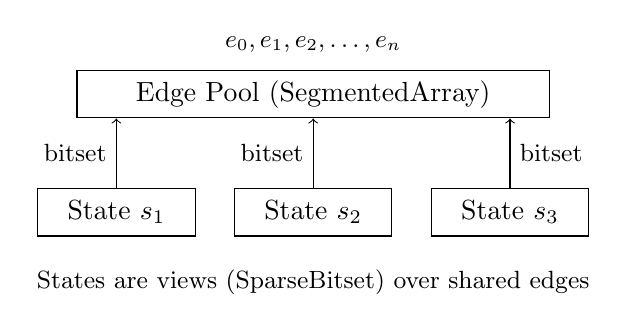
\begin{tikzpicture}[
    box/.style={rectangle, draw, minimum width=2cm, minimum height=0.6cm},
    label/.style={font=\small}
]
% Edge Pool
\node[box, minimum width=6cm] (pool) at (0,0) {Edge Pool (SegmentedArray)};
\node[label, above=0.1cm of pool] {$e_0, e_1, e_2, \ldots, e_n$};

% States
\node[box] (s1) at (-2.5,-1.5) {State $s_1$};
\node[box] (s2) at (0,-1.5) {State $s_2$};
\node[box] (s3) at (2.5,-1.5) {State $s_3$};

% Arrows
\draw[->] (s1.north) -- node[left, label] {bitset} (s1.north |- pool.south);
\draw[->] (s2.north) -- node[left, label] {bitset} (s2.north |- pool.south);
\draw[->] (s3.north) -- node[right, label] {bitset} (s3.north |- pool.south);

% Legend
\node[label, below=0.3cm of s2] {States are views (SparseBitset) over shared edges};
\end{tikzpicture}
\caption{Unified edge storage with state views}
\label{fig:storage}
\end{figure}

The bitset is divided into chunks, and a child shares its parent's chunks until it changes one, at
which point that chunk is copied. A rewrite that changes a few edges allocates a few chunks, and
shared chunks are never modified, so readers of the parent are unaffected by the child.
Table~\ref{tab:t3-deheap} gives the arena bytes of each corpus workload. Appendix~\ref{app:data-structures}
specifies the lock-free structures, their per-operation costs, the memory model, and the behavior
at configured limits.

\subsection{Allocation}
\label{sec:allocation}

Evolution allocates from per-worker arenas. Each worker bumps a pointer into blocks it owns, so
allocation during matching and rewriting needs no synchronization, and memory is freed in bulk by
resetting the arena. The global allocator is called only to obtain those blocks:
Table~\ref{tab:t3-deheap} reports $455$ to $475$ calls for an entire run, which on the largest
workloads is $0.007$ calls per event.

\subsection{Static Rule Analysis}
\label{sec:static-analysis}
\label{sec:rule-analysis}

When a rule is added, the engine computes properties that follow from its patterns alone and uses
them to choose a strategy. For each rule it records the difference in edge count between the two
sides, which says whether states grow; the number of new vertices the right-hand side introduces;
and the left-hand side's arities. Treating the left-hand side as a conjunctive query, it computes
whether the query is acyclic and an integral edge cover $\rho$, which bounds the matches in a state
of $N$ edges by $N^{\rho}$. The bound is tight when the query is acyclic, and is used only as an
upper bound otherwise.

Each predicate is sound in one direction. The branching test is an over-approximation: a negative
answer means no two matches can ever share a consumed edge, and a positive answer means only that
this has not been ruled out. The engine acts only on the negative answer: the branchial relation
is then empty for every initial state, and the engine returns it empty without computing it. No
analysis here decides termination, finiteness of the reachable set, or confluence, which are
undecidable for rewriting systems of this kind.

\subsection{Determinism Contract}
\label{sec:determinism}

The state set, the event set and the causal and branchial relations are a deterministic function of
the rules, the initial state, the step count and the options. They do not depend on the number of
worker threads, the order in which tasks run, or whether quotient exploration is enabled. State and
event identifiers are allocated in arrival order and vary between runs; the observables are defined
over canonical identities. A determinism gate checks this across thread counts and seeds: it
fingerprints the expanded state set, the multiset of (input, output, rule) transitions, and the
causal and branchial relations separately, and reports which component differs and under which
configuration. The components are compared separately because the causal relation can differ by a
single edge while the others agree.

The count caps \textsc{MaxStatesPerStep} and \textsc{MaxSuccessorStatesPerParent} are outside the
contract. They admit states until a counter reaches the cap, so which states are admitted depends
on arrival order and varies with the worker count. Making them schedule-independent would require
holding every candidate at a depth until the depth is complete, which is a barrier. A capped run
guarantees the count at every worker count, not which states make it up.

\subsection{Depth Semantics and Termination}
\label{sec:depth}

The step budget applies to the \emph{shortest} path from an initial state to a canonical state, not
to the path along which the state was first reached. Under concurrency a state can be reached first
along a long path and later along a short one, so a budget on arrival depth would include or exclude
states according to which path won the race, and the explored set would vary with the thread count.

The engine therefore \emph{relaxes} depths: when a state is reached along a path shorter than its
recorded depth, the recorded depth is lowered and the change is propagated to its children, and
from them onward. This terminates because each accepted change lowers a depth, which is bounded
below by zero. A state is matched at most once however often its depth is lowered, because the
claim that admits a state to expansion is separate from its depth.

Relaxation races the registration of a new child. Registration publishes the child and then reads
the parent's depth; relaxation lowers the depth and then scans the child list. Sequentially
consistent fences on both sides rule out the case where the scan misses the child and the read
misses the lowered depth, so a child always sees its parent's current minimum depth. A state past
the budget stays on the frontier without being claimed, so a shorter path found later can still
bring it within the budget. A state is claimed against the same bound its match task is admitted
under, so a claimed state is never left unmatched.

Work budgets are taken by compare-and-swap. An increment followed by a rollback would briefly
publish a count above the limit, and a thread reading the count at that moment would prune work
that another schedule keeps.

Termination is detected without a barrier: a depth is complete when it has no live work and the
depth below it is complete. This suffices because a task at depth $d$ only creates work at depths
above $d$, so once depth $d-1$ is complete nothing new can arrive at $d$.

\subsection{Transitive Reduction of the Causal Graph}
\label{sec:tr}

The causal graph has an edge for every dependency between events, including those implied by
longer paths. Its transitive reduction removes an edge $p \to c$ whenever a path
$p \rightsquigarrow c$ of length greater than one exists; on an acyclic graph the reduction is
unique.

Goranci et al.~\cite{goranci2025dynamic} give the first fully dynamic algorithms for the transitive
reduction of a general directed graph under insertions and deletions, in $\BigO(m + n\log n)$
amortized update time, and $\BigO(m + n^{1.585})$ worst case with fast matrix multiplication. This
engine's case is simpler in two ways. First, causal edges are only inserted, so an edge dropped as implied
never needs to be reconsidered. Second, edges arrive in topological order, because an event's producers
exist before the event, so when an edge $(p,c)$ arrives the closure below $p$ is final. The
procedure below is the specialization of the problem to this case.

\paragraph{Online maintenance.}
The reduction is kept up to date after every insertion, because a session
(Section~\ref{sec:sessions}) can be queried between steps, and because building the full relation
first would allocate the transitive closure that the reduction avoids.

\paragraph{Procedure (Algorithm~\ref{alg:tr}).}
Let $e = (p, c)$ be a new causal edge: event $p$ produced an edge that event $c$ consumed. If $c$ is
already reachable from $p$ through retained edges, $e$ is implied and dropped; otherwise it is
retained. A retained edge never needs to be removed later. A consumer's incoming edges are added by
its own worker in descending producer order, and an ancestor's id is always smaller than its
descendant's. A retained $(p', c)$ could become implied only through a path
$p' \rightarrow \cdots \rightarrow x \rightarrow c$. If $(x, c)$ arrived first, the query for
$(p', c)$ saw the path and dropped the edge; if $(x, c)$ arrived later, then $x < p'$ by the
descending order, while reachability from $p'$ requires $p' < x$, a contradiction. Hence deciding each
edge once on arrival gives the exact reduction. The descending order also makes queries cheap,
because the closure from nearer producers is built before farther ones are tested, and it needs no
sorting, because events are numbered in creation order.

\begin{algorithm}[htbp]
\caption{Online Transitive Reduction (insertion-only)}
\label{alg:tr}
\begin{algorithmic}[1]
\Procedure{ConsumeEdges}{event $c$, producers $P$}
    \ForAll{$p \in P$ in descending event id}
        \If{$c$ reachable from $p$ via retained edges}
            \State drop $(p, c)$ as implied
        \Else
            \State retain $(p, c)$
        \EndIf
    \EndFor
\EndProcedure
\end{algorithmic}
\end{algorithm}

\paragraph{Order independence.}
The retained edge set must depend only on the causal DAG, not on the order in which concurrent
workers insert edges; the determinism gate checks this across thread counts and seeds. Full capture
meets it through the arrival order above: each consumer's edges are added by its own worker, in
descending producer order, after its producers' edges are complete, and under that order the
decision on arrival is exact however consumers interleave. The quotient reconstruction adds edges
between canonical event ids, which are not ordered this way, so it stores the relation unreduced
and reduces it when it is read; a finite DAG has one transitive reduction, so the result depends
only on the stored edges.

Only the causal graph is reduced. States, events and the branchial relation are not.



\section{Exploration Strategies}
\label{sec:exploration}

Exhaustive evolution becomes infeasible at moderate depth, and a caller may need only part of
it. The engine has four independent ways to limit an exploration, and they can be combined:

\begin{itemize}
\item \textbf{Caps.} A total state count, a total event count, a count of states admitted per step
      (\textsc{MaxStatesPerStep}) and a count of successors per parent
      (\textsc{MaxSuccessorStatesPerParent}). Each is an atomic counter, so the count retained is
      exact at every worker count; which states fill a cap depends on arrival order
      (Section~\ref{sec:determinism}). A run that reaches a cap returns what it computed with a
      warning (Section~\ref{sec:capacity}).
\item \textbf{Sampling.} Per-rule transition rates and a per-state match cap keep a subset of
      transitions chosen by keyed pseudorandom draws, so the sample is reproducible for a seed at
      every worker count (Section~\ref{sec:sampling}).
\item \textbf{Quotient exploration} (Section~\ref{sec:quotient}) expands one state per isomorphism
      class and reconstructs the raw relations exactly.
\item \textbf{Steering.} A session (Section~\ref{sec:sessions}) reports the frontier after each
      step, and the next step can be restricted to part of it; the rest stays on the frontier.
\end{itemize}

Caps and steering compute a subset exactly; sampling computes a random subset; quotient exploration
computes the full result and expands less. The step budget bounds all four, and the reported
frontier records where each stopped.
\label{sec:pruning}

\subsection{Quotient Exploration}
\label{sec:quotient}

In full expansion every raw state is expanded, so a state reached along $k$ histories is matched $k$
times, although canonicalization has already shown the repeats find no new states. Quotient
exploration expands only one state per isomorphism class, at the shallowest depth the class was
reached. Every equivalent state is still created and its incoming event recorded.
Table~\ref{tab:t6-quotient} gives events produced, causal edges and wall time for both modes by
depth. Both modes give the same canonical state set. The causal and branchial relations are
defined over raw events, which quotient exploration does not all produce, so they are
reconstructed.

The number of raw events is recovered by a forward summation. Under exact identity the canonical
states graph has cycles, because a canonical state recurs at several depths, but its unrolling by
depth is acyclic, and the multiplicity of each (canonical state, depth) pair satisfies
\begin{align}
  \mathrm{mult}[s_0, 0] &= 1, \nonumber\\
  \mathrm{mult}[c, k{+}1] &\mathrel{+}= \mathrm{mult}[s, k]\cdot w(s \to c),
  \label{eq:mult}
\end{align}
summed over the transitions into $c$; the raw event count is $\sum \mathrm{mult}$. This takes time
polynomial in the number of (canonical state, depth) pairs.

The raw events and relations themselves are recovered by replaying each class's expansion against
every instance of the class. The expansion is recorded once, in the \emph{frame} of the first raw
state that reached the class: each match found on that state is stored as indices into the frame's
edges. Another raw state of the class is aligned onto the frame by the canonical edge ranks from
its own IR run; this alignment is an isomorphism, defined up to an automorphism, so it maps matches
to matches. The edge orbits from the same IR pass distinguish edge roles within a class
(Section~\ref{sec:ir}), so no further canonicalization is needed. An \emph{instance} of a class at
depth $k$ is a vector holding one producer event per frame slot. Applying a recorded match to an
instance creates one raw event; adds a causal edge from the producer of each consumed slot, in
descending producer order so that the online reduction of Section~\ref{sec:tr} stays exact; adds a
branchial pair with each earlier application at the same instance whose consumed slots overlap;
and creates a child instance at depth $k+1$, in which surviving slots keep their producer and
produced slots take the new event. Instances and recorded matches arrive concurrently, so each new
instance replays every match already recorded for its class, each new match is replayed against
every instance already present, and each (instance, match) pair is claimed exactly once. A replayed
event has two identities: the triple (source class, target class, rule), which is an isomorphism
invariant used for comparisons across runs and engines, and the run's event identity.

The reconstruction creates as many instances as the full system has raw states. On a two-rule set
whose canonical state count grows linearly with depth (three to eight states at depths two to
seven), the raw system has 146,599 states at depth six, and the reconstruction's cost follows that
count. There, quotient exploration visited 49 raw states against full capture's 146,599 and ran 65
times faster.

The reconstruction runs only when the causal relation, the branchial relation or the raw event set
is requested; a run that asks for canonical states alone skips it. Every worker takes part in it,
and its total cycle count grows with the thread count (Section~\ref{sec:limitations}).

\subsection{Sampled Exploration}
\label{sec:sampling}

The engine has two samplers. The \emph{transition rate} keeps each candidate transition
independently with a fixed probability, multiplied by a per-rule weight; the number of children a
state keeps is then a random variable with the thinned distribution of the full one. The
\emph{per-state match cap} keeps at most $k$ of each state's matches for each rule. Both choose by a
pseudorandom value computed from the transition's canonical identity and the seed, so the same seed
gives the same sample at any thread count (Section~\ref{sec:determinism}).

\paragraph{Choosing the rate.}
A fixed rate compounds with depth: a path of length $L$ survives with probability $q^L$. On the
workloads measured, rates of $1/8$ and $1/4$ end the evolution within the first step and $1/2$
leaves it growing, so the usable range is narrow and depends on the rule's branching factor. While
a rate or weight below one is in effect, a state whose own draws all fail keeps its
lowest-ranked own transition, so the evolution does not die out; a state with no matches of its
own has no such fallback.

\paragraph{The per-state cap.}
Samples from different seeds do not add up to the exhaustive system, because a transition can be
drawn only if its source state was created, which required an earlier draw to succeed. The
per-state cap keeps at least one transition at every state it reaches, so each seed covers a
connected skeleton, and different seeds keep different skeletons. The cap chooses $k$ of a state's
$M$ matches by rank once the state's matching is complete, because choosing $k$ of $M$ needs all
$M$; choosing by arrival order would make the result depend on the schedule. A match forwarded
from an ancestor can arrive after the state's matching is complete, so a run under the cap turns
match forwarding off and each state finds all of its matches itself.

\paragraph{Per-state and per-transition draws.}
Under full capture each raw state is created by exactly one event, so a draw per new state and a
draw per transition are the same draw. Under quotient exploration a canonical state has many
incoming transitions, and the two differ.

\paragraph{No barrier.}
A decision to keep a match is final once the match is rewritten, so a sample must be complete
before its members are rewritten. A sample drawn from a whole evolution step would be complete only
when every worker finished the step, which is a global barrier. The engine therefore samples only
over populations that complete locally: a state's matches for one rule are complete when that
state's matching tasks have all finished, which the engine detects without looking at any other
state.

\subsection{Sessions}
\label{sec:sessions}

Evolution is also available as a session: it is opened on a rule set and an initial state, advanced
by a number of steps, queried for any derived structure, and closed. The frontier is kept between
steps, so each step continues the existing evolution instead of starting again.

The frontier is stored separately from the canonical identity map. The map records which states
have been seen; the frontier records the states and pending rewrites that the step budget stopped,
together with the depth each waits at.

Every session reply reports the frontier, and a step may name part of it. The named entries are
advanced and the others stay on the frontier. A step that names no entries advances the whole
evolution to the new total depth, and gives the same result as a single run to that depth. A step
that names entries advances each of them by the requested number of steps from the depth it waits
at, so entries at different depths each advance by the same amount. Naming a state that is not on
the frontier is an error. A continuable run stopped by a state or event limit keeps the work the
limit cut short on the frontier (Section~\ref{sec:capacity}). Both devices implement this interface.



\section{GPU Acceleration}
\label{sec:gpu}

Multiway evolution is an irregular workload for a GPU. The frontier's width depends on the data
and is not known until the step that produces it, and every new state must be canonicalized before
it can be compared with others, by the same IR code the host runs, whose control flow depends on
the data. The kernel spreads IR's loops across the lanes of a warp where the loops allow it. A
kernel launch per step would put a host round trip between every stage, so the engine runs one
resident kernel that keeps the frontier on the device for the whole evolution.
Appendix~\ref{app:gpu-impl} specifies the device canonicalization, matching, work queues,
termination and memory management.

\subsection{Resident Kernel}

A kernel launch has a fixed cost, which dominates the early steps of an evolution, where the
frontier is small. The engine runs a single persistent kernel for the whole evolution, with the
frontier, the match queues and the epoch counter kept in device memory, so a step costs a
device-side barrier rather than a launch. The match, rewrite and state queues are resident, and a
new state becomes a match task without returning to the host. The resident kernel is
$\PersistentSpeedupFour\times$ faster than a per-step \texttt{evolve()} at depth four, and the two
take the same time from depth \PersistentTieDepthWord{} on, where the evolution itself outweighs
the launch cost (Section~\ref{sec:benchmarks}).

One block matches one (state, rule) pair, and its threads divide the candidates for the first
pattern edge. Later pattern edges take their candidates from a vertex index through a variable
that is already bound, as described in Appendix~\ref{app:gpu-impl}.

\subsection{Design Constraints}
\label{sec:gpu-constraint}

Nothing crosses the host--device boundary while the kernel runs. Rules and the initial state are
uploaded and the queues seeded before the launch, and results are read after it; in between, the
device decides what work exists, which worker takes it, and when the evolution has finished. Any
round trip during the run would cost as much as the per-step round trip the design removes.

This has two consequences.

\emph{The kernel cannot grow a pool.} Growing a pool needs a host allocation. When a pool
overflows, the kernel records the overflow and returns the work completed so far; the host then
re-runs the evolution with doubled capacities, up to eight times, and returns the last partial
result with a warning if it still overflows (Section~\ref{sec:capacity}).

\emph{Canonicalizer scratch cannot be sized from a batch.} The resident kernel has no batch: states
arrive continuously and the largest is not known until the run ends. Scratch pre-sized from a
configured maximum, with a coarser hash above it, would let two non-isomorphic states share a key
whenever one was too large to canonicalize exactly. Instead each state takes scratch from a
device-side arena, sized from its own vertex, edge and occurrence counts. Exhausting the arena is a
capacity overflow, handled as above; the exact path never falls back to a coarser identity.


\section{Experimental Evaluation}
\label{sec:benchmarks}

The evaluation answers five questions.

\begin{description}
\item[Q1 (correctness).] Is state identity exact (two states identified if and only if they are
isomorphic) on every corpus workload, checked against an independent oracle?
(Table~\ref{tab:t1-exactness})
\item[Q2 (speed against the reference).] How does evolution time compare with the Wolfram
implementation of the same computation, and how does the ratio change with depth?
(Table~\ref{tab:t2-speedup}, Figure~\ref{fig:speedup})
\item[Q3 (parallel scaling).] How does evolution time change with the worker count, does that
depend on the rule, and what limits it? (Tables~\ref{tab:t8-scaling}, \ref{tab:t12-shapes},
\ref{tab:t13-memory}; Figure~\ref{fig:scaling})
\item[Q4 (device).] Where is the GPU faster than the CPU, and at what grid size does it saturate?
(Tables~\ref{tab:t7-gpu}, \ref{tab:t7b-gpu-corpus}, \ref{tab:t11-saturation})
\item[Q5 (attribution).] Which parts of the engine account for its speed, and does any of them
change the result? (Tables~\ref{tab:t9-ablation}, \ref{tab:t6-quotient}, \ref{tab:event-canon})
\end{description}

\subsection{Experimental Setup}

\begin{description}
\item[Hardware:] AMD EPYC 9174F (16 cores, 32 threads, one socket), 503\,GB RAM, NVIDIA RTX 4090 (24\,GB, compute capability 8.9), on bare metal. The cores are identical, so speedups divide comparable quantities. Workers are placed in the engine's default order, read from the cache topology at start-up: the cores of one last-level-cache domain and their SMT siblings are filled before the next domain is used. The Wolfram comparison of Table~\ref{tab:t2-speedup} needs a licensed Wolfram kernel and ran on a different machine, an Intel i9-14900K.
\item[Software:] Ubuntu 24.04, Linux 6.8, GCC with C++20, CUDA 12.0, Wolfram Language 14.3.
\item[Workloads:] A corpus of 17 workloads covering rule types (single and multiple rules; productive, idempotent, reductive and mixed-arity rules; several initial-state shapes), and deeper runs of the canonical Wolfram rule $\{\{x,y,z\}\} \to \{\{x,y,w\},\{y,z,w\}\}$ for the scaling and GPU measurements.
\item[Methodology:] Wall times are medians over repeated runs on an otherwise idle machine, and the two arms of any comparison are measured in the same session, because run-to-run variation on this machine exceeds many of the effects reported. Counts, instruction counts and \texttt{getrusage} figures are deterministic and come from a single run. The left-hand-side sweep of Figure~\ref{fig:lhs-scaling} reports the \emph{minimum} of its repeats, because interference from other load can only slow a run, and it starts a timed run only when the machine is idle.
\end{description}

\subsection{Correctness and Memory Footprint}
Every corpus workload is evolved single-threaded in the exact mode to the depth listed with it,
chosen so that the brute-force check stays tractable; depths differ between rows, so counts are
comparable within a column but not across rows. Its canonical state set, event set, causal
relation and branchial relation are compared with the reference implementation
(Table~\ref{tab:t1-exactness}), and each state set is checked against a brute-force isomorphism
oracle. All seventeen workloads agree exactly.

Table~\ref{tab:t3-deheap} gives the memory the same runs use. Arena bytes come from the arena's own
counter, which is deterministic, rather than from the resident set size. The global allocator is
called $455$ to $475$ times per run, for set-up that does not grow with the evolution, so calls
per event fall from $456$ on the smallest workload to $0.007$ on the largest.

\begin{table}[htbp]
\centering
\caption{Canonical states, events, causal edges and branchial edges for each corpus workload;
the brute-force oracle confirms every workload.}
\label{tab:t1-exactness}
% GENERATED by tools/dev/paper_tables.py -- do not edit.
% commit e6f5e5ef | Intel(R) Core(TM) i9-14900K, 20 GB RAM, Linux 5.15.167.4-microsoft-standard-WSL2 | source: tools/cost_matrix.cpp
%% arena bytes, all artifacts / neither relation: 286829596 / 179900636  (37.3% of the arena is the causal and branchial graphs)
\resizebox{\ifdim\width>\linewidth\linewidth\else\width\fi}{!}{%
\begin{tabular}{llrrrrrrrl}
\toprule
Workload & Class & Canon.\ states & Events & Causal & Branchial & Arena B & Heap B & Heap allocs & Exactness \\
\midrule
binary-growth & productive/arity2 & 874 & 36 & 873 & 872 & 0 & 1397512 & 3116132 & exact \\
wolfram-2to4 & productive/arity2 & 127 & 45 & 126 & 184 & 111 & 655024 & 1498684 & exact \\
triangle & productive/mixed-conn & 125 & 36 & 124 & 192 & 249 & 645784 & 1515100 & exact \\
reductive-2to1 & reductive/arity2 & 16 & 4 & 15 & 12 & 5 & 530968 & 1497212 & exact \\
idempotent-2to2 & idempotent/arity2 & 7 & 1 & 6 & 10 & 0 & 507920 & 1497164 & exact \\
self-loop & self-loop/arity2 & 2 & 2 & 1 & 0 & 0 & 363336 & 1251380 & exact \\
mixed-arity & mixed-arity & 7 & 7 & 6 & 5 & 0 & 440712 & 1513572 & exact \\
arity3-growth & arity3 & 154 & 65 & 153 & 152 & 0 & 542224 & 1498740 & exact \\
disconnected-lhs & disconnected & 127 & 1 & 126 & 248 & 63 & 634032 & 1497458 & exact \\
arity4-growth & arity4 & 34 & 23 & 33 & 32 & 0 & 460552 & 1497060 & exact \\
mixed-arity-lhs & mixed-arity/join & 2 & 2 & 1 & 0 & 0 & 380168 & 1251356 & exact \\
mixed-arity-init & mixed-arity/init & 5 & 4 & 4 & 0 & 0 & 398000 & 1513564 & exact \\
arity3-to-2 & arity-reductive & 5 & 4 & 4 & 0 & 0 & 398172 & 1513596 & exact \\
arity1-with-binary & arity1/mixed & 2 & 2 & 1 & 0 & 0 & 380152 & 1251340 & exact \\
cycle4-automorphic & automorphism & 68185 & 7 & 68184 & 109992 & 68184 & 179140120 & 201283020 & exact \\
star4-automorphic & automorphism & 68185 & 201 & 68184 & 56360 & 0 & 99249768 & 118459724 & exact \\
multi-rule & multi-rule & 238 & 36 & 237 & 214 & 108 & 705152 & 2060060 & exact \\
\bottomrule
\end{tabular}
}

\end{table}

\begin{table}[htbp]
\centering
\caption{Arena bytes, heap bytes, and global \texttt{operator new} calls during
evolution, per corpus workload, ordered by work performed.}
\label{tab:t3-deheap}
% GENERATED by tools/dev/paper_tables.py -- do not edit.
% commit e6f5e5ef | Intel(R) Core(TM) i9-14900K, 20 GB RAM, Linux 5.15.167.4-microsoft-standard-WSL2 | source: tools/cost_matrix.cpp
\resizebox{\ifdim\width>\linewidth\linewidth\else\width\fi}{!}{%
\begin{tabular}{lrrrrr}
\toprule
Workload & Canon.\ states & Events & Arena B & Heap allocs & Allocs per event \\
\midrule
idempotent-2to2 & 7 & 1 & 0 & 1497164 & 1497164.0000 \\
disconnected-lhs & 127 & 1 & 63 & 1497458 & 1497458.0000 \\
self-loop & 2 & 2 & 0 & 1251380 & 625690.0000 \\
mixed-arity-lhs & 2 & 2 & 0 & 1251356 & 625678.0000 \\
arity1-with-binary & 2 & 2 & 0 & 1251340 & 625670.0000 \\
reductive-2to1 & 16 & 4 & 5 & 1497212 & 374303.0000 \\
mixed-arity-init & 5 & 4 & 0 & 1513564 & 378391.0000 \\
arity3-to-2 & 5 & 4 & 0 & 1513596 & 378399.0000 \\
mixed-arity & 7 & 7 & 0 & 1513572 & 216224.5714 \\
cycle4-automorphic & 68185 & 7 & 68184 & 201283020 & 28754717.1429 \\
arity4-growth & 34 & 23 & 0 & 1497060 & 65089.5652 \\
binary-growth & 874 & 36 & 0 & 3116132 & 86559.2222 \\
triangle & 125 & 36 & 249 & 1515100 & 42086.1111 \\
multi-rule & 238 & 36 & 108 & 2060060 & 57223.8889 \\
wolfram-2to4 & 127 & 45 & 111 & 1498684 & 33304.0889 \\
arity3-growth & 154 & 65 & 0 & 1498740 & 23057.5385 \\
star4-automorphic & 68185 & 201 & 0 & 118459724 & 589351.8607 \\
\bottomrule
\end{tabular}
}

\end{table}

\begin{figure}[htbp]
\centering
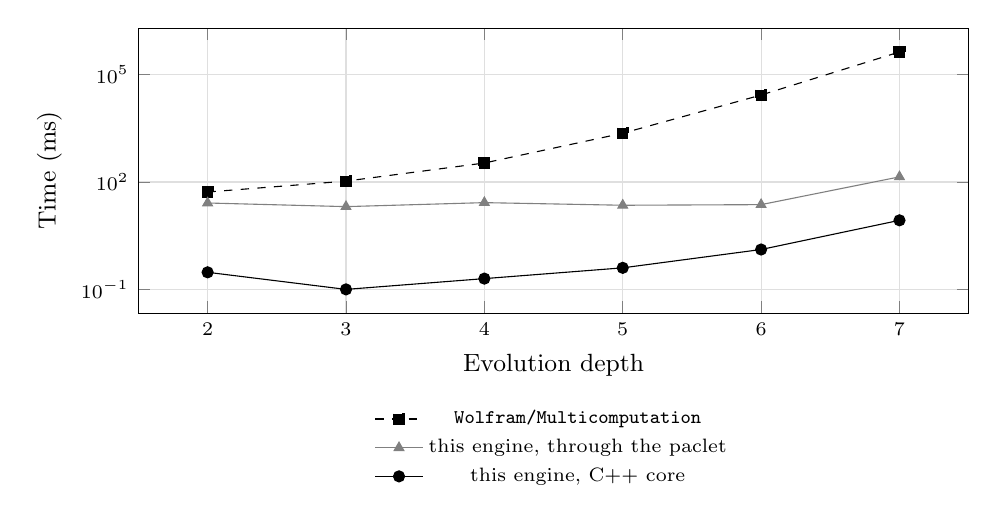
\begin{tikzpicture}
\begin{axis}[
    width=\linewidth, height=5.2cm,
    xlabel={Evolution depth}, ylabel={Time (ms)},
    ymode=log, xtick={2,3,4,5,6,7}, grid=major, grid style={gray!25},
    legend style={font=\scriptsize, at={(0.5,-0.30)}, anchor=north, legend columns=1,
                  draw=none, fill=none},
    label style={font=\small}, tick label style={font=\scriptsize},
]
% GENERATED by tools/dev/paper_tables.py -- do not edit.
% commit e6f26a9d | measured on Intel(R) Core(TM) i9-14900K, 31 GB RAM, Linux 5.15.167.4-microsoft-standard-WSL2 | load at start 0.19/0.23 (1m/15m) | source: reference/bench_authority.wls + tools/quotient_reconstruction_cost_probe.cpp (Wolfram kernel on cpu mask FFFF)
% paclet versions: HypergraphRewriting 1.0.0, SetReplace 0.3.196, Wolfram/Multicomputation 0.1.8

\addplot[mark=square*, black, dashed] coordinates {(2,52.5)(3,105.7)(4,339.1)(5,2298.6)(6,26830.7)(7,428264.0)};
\addlegendentry{\texttt{Wolfram/\allowbreak Multicomputation}}
\addplot[mark=triangle*, black!50] coordinates {(2,25.9)(3,20.5)(4,26.5)(5,22.4)(6,23.3)(7,139.0)};
\addlegendentry{this engine, through the paclet}
\addplot[mark=*, black] coordinates {(2,0.3)(3,0.1)(4,0.2)(5,0.4)(6,1.3)(7,8.5)};
\addlegendentry{this engine, C++ core}

\end{axis}
\end{tikzpicture}
\caption{Evolution time against depth for \texttt{MultiwaySystem}, the engine through the paclet,
and the engine's C++ core, on the same rule and initial state; all three give the same state and
causal-edge counts at every depth. The gap between the first and last series is the speedup of
Table~\ref{tab:t2-speedup}; the gap between the last two is the cost of the Wolfram interface.}
\label{fig:speedup}
\end{figure}

\subsection{Wall-Time Speedup}
The timed comparison is against the \texttt{Wolfram/\allowbreak Multicomputation} paclet's
\texttt{MultiwaySystem}, the published implementation of the same computation. The reference
implementation (Section~\ref{sec:background}) checks that all three agree on state and causal-edge
counts at every depth, and they do; its time is not reported. From depth four to seven the
engine's core is $\SpeedupAtLowDepth\times$ to $\SpeedupAtHighDepth\times$ faster than
\texttt{MultiwaySystem}, and the ratio increases with each depth. The depth-two time includes
\texttt{MultiwaySystem}'s one-time initialization, and at depths two to five the engine takes a
fraction of a millisecond, close to the timer's resolution, so the ratios at those depths are
lower bounds. At depth seven the engine takes $\CoreDeepMs$\,ms and
\texttt{MultiwaySystem} $\AuthorityDeepSeconds$\,s, both well above the resolution.

Each side is timed through its user-facing interface. Every \texttt{MultiwaySystem} property
returns a Wolfram \texttt{Graph} (\texttt{StatesGraph}, \texttt{CausalGraph},
\texttt{EvolutionGraph} and others), so its time includes building graphs. The engine is timed
twice: through its C++ API, and through the paclet, which serializes the request to the engine's
process over WXF, evolves, and builds the same kind of Wolfram structures on return. The difference
between the two is the cost of the Wolfram interface on the same computation: at depth
\SpeedupHighDepth{} it turns $\CoreDeepMs$\,ms into $\PacletDeepSeconds$\,s, a factor of
$\PacletOverheadDeep\times$. Through the paclet the engine is still $\PacletVsAuthorityDeep\times$
faster than \texttt{MultiwaySystem}.

\begin{table*}[htbp]
\centering
\caption{Wall time by depth against \texttt{MultiwaySystem} on
\texttt{wolfram-2to4}: $\{\{1,2\},\{2,3\}\} \to
\{\{1,2\},\{2,4\},\{4,3\}\}$ from $\{\{1,2\},\{2,3\}\}$. The engine is timed through its C++ API
and through the paclet (WXF and Wolfram structure construction included); the speedup column
divides \texttt{MultiwaySystem}'s time by the C++ core's. The reference implementation checks the
counts and is not timed.}
\label{tab:t2-speedup}
% GENERATED by tools/dev/paper_tables.py -- do not edit.
% commit e6f26a9d | measured on Intel(R) Core(TM) i9-14900K, 31 GB RAM, Linux 5.15.167.4-microsoft-standard-WSL2 | load at start 0.19/0.23 (1m/15m) | source: reference/bench_authority.wls + tools/quotient_reconstruction_cost_probe.cpp (Wolfram kernel on cpu mask FFFF)
% paclet versions: HypergraphRewriting 1.0.0, SetReplace 0.3.196, Wolfram/Multicomputation 0.1.8
{\footnotesize\setlength{\tabcolsep}{4pt}%
\resizebox{\ifdim\width>\linewidth\linewidth\else\width\fi}{!}{%
\begin{tabular}{rrrrrr}
\toprule
Depth & States & \texttt{MultiwaySystem} ms & Engine ms (paclet) & Engine ms (C++ core) & Speedup (core vs.\ \texttt{MultiwaySystem}) \\
\midrule
2 & 3 & 52.5 & 25.9 & 0.3 & 175$\times$ \\
3 & 4 & 105.7 & 20.5 & 0.1 & 1057$\times$ \\
4 & 5 & 339.1 & 26.5 & 0.2 & 1696$\times$ \\
5 & 6 & 2298.6 & 22.4 & 0.4 & 5746$\times$ \\
6 & 7 & 26830.7 & 23.3 & 1.3 & 20639$\times$ \\
7 & 8 & 428264.0 & 139.0 & 8.5 & 50384$\times$ \\
\bottomrule
\end{tabular}
}}

\end{table*}

\subsection{Quotient Exploration}
Quotient exploration expands each canonical state once, at its shallowest depth, so it produces far
fewer events than full expansion, and both give the same canonical state set
(Table~\ref{tab:t6-quotient}). At depth seven quotient exploration produces $28$ events where full
expansion produces $5{,}913$, and the reconstruction recovers all $5{,}913$, with their causal
edges and branchial pairs, from those $28$. The reconstruction's cost is below the resolution of
this measurement: at most depths the \texttt{quot.+recon} time is at or below the \texttt{quot.}
time, which is run-to-run variation on sub-millisecond timings.

\begin{table}[htbp]
\centering
\caption{Events and wall time, quotient exploration against full expansion, by depth on the
Wolfram rule; at every depth the reconstruction gives full expansion's event and causal counts
exactly.}
\label{tab:t6-quotient}
% GENERATED by tools/dev/paper_tables.py -- do not edit.
% commit 769b12ba | Intel(R) Core(TM) i9-14900K, 20 GB RAM, Linux 5.15.167.4-microsoft-standard-WSL2 | source: tools/quotient_reconstruction_cost_probe.cpp
\resizebox{\ifdim\width>\linewidth\linewidth\else\width\fi}{!}{%
\begin{tabular}{rrrrrrrrl}
\toprule
Depth & Events (full) & Causal (full) & ms (full) & Events (quot.) & ms (quot.) & Events (quot.+recon) & ms (quot.+recon) & Exact \\
\midrule
2 & 3 & 4 & 0.3 & 3 & 0.2 & 3 & 0.2 & exact \\
3 & 9 & 16 & 0.1 & 6 & 0.2 & 9 & 0.2 & exact \\
4 & 33 & 64 & 0.1 & 10 & 0.2 & 33 & 0.2 & exact \\
5 & 153 & 304 & 0.3 & 15 & 0.2 & 153 & 0.2 & exact \\
6 & 873 & 1744 & 1.6 & 21 & 0.4 & 873 & 0.4 & exact \\
7 & 5913 & 11824 & 16.0 & 28 & 1.7 & 5913 & 1.8 & exact \\
\bottomrule
\end{tabular}
}

\end{table}

\begin{figure}[htbp]
\centering
\begin{subfigure}{\linewidth}
\centering
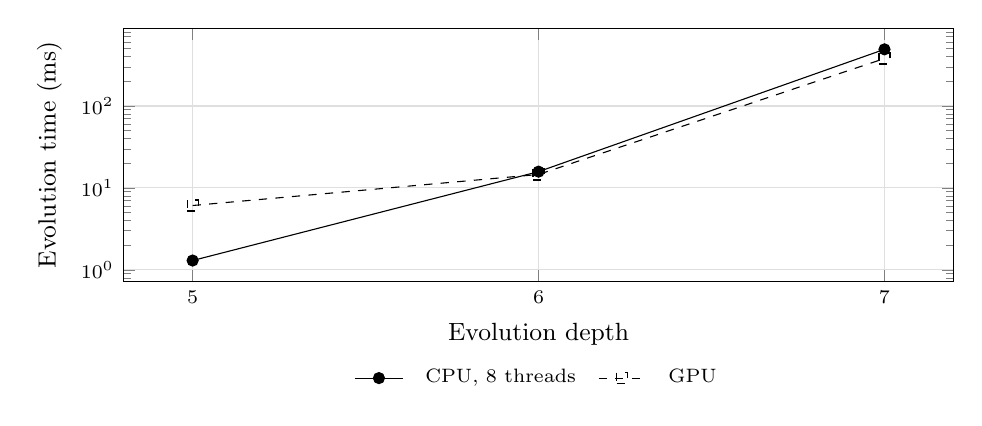
\begin{tikzpicture}
\begin{axis}[
    width=\linewidth, height=4.8cm,
    xlabel={Evolution depth}, ylabel={Evolution time (ms)},
    ymode=log, xtick={4,5,6,7,8,9}, grid=major, grid style={gray!25},
    legend style={font=\scriptsize, at={(0.5,-0.30)}, anchor=north, legend columns=2,
                  draw=none, fill=none, column sep=6pt},
    label style={font=\small}, tick label style={font=\scriptsize},
]
% GENERATED by tools/dev/paper_tables.py -- do not edit.
% commit 1d5bc1c9 | Intel(R) Core(TM) i9-14900K, 20 GB RAM, Linux 5.15.167.4-microsoft-standard-WSL2 | source: tools/bench_cpu_evolve.cpp + tools/bench_gpu_evolve.cpp

\addplot[mark=*, black] coordinates {(5,1.3)(6,15.8)(7,491.3)};
\addlegendentry{CPU, 8 threads}
\addplot[mark=square, black, dashed] coordinates {(5,6.1)(6,14.6)(7,379.9)};
\addlegendentry{GPU}

\end{axis}
\end{tikzpicture}
\caption{Evolution time against depth, the device against eight CPU threads
(Table~\ref{tab:t7-gpu}).}
\end{subfigure}

\vspace{2mm}
\begin{subfigure}{\linewidth}
\centering
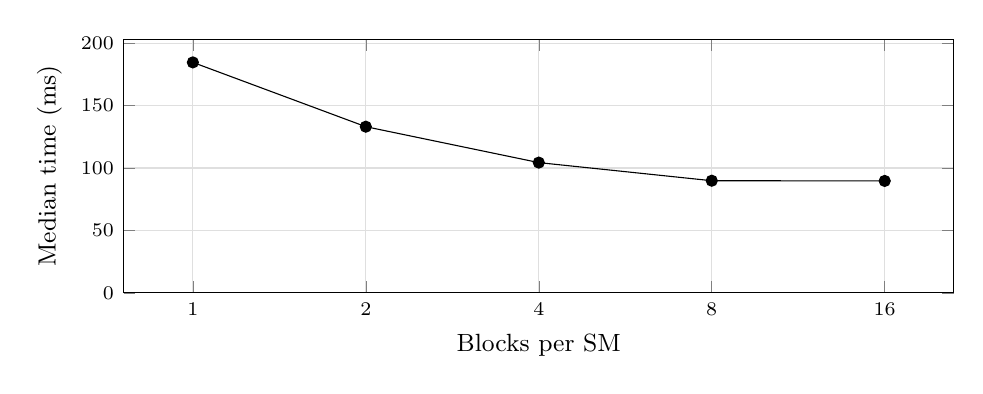
\begin{tikzpicture}
\begin{axis}[
    width=\linewidth, height=4.8cm,
    xlabel={Blocks per SM}, ylabel={Median time (ms)},
    xmode=log, log basis x=2, xtick={1,2,4,8,16}, xticklabels={1,2,4,8,16},
    ymin=0, grid=major, grid style={gray!25},
    label style={font=\small}, tick label style={font=\scriptsize},
]
% GENERATED by tools/dev/paper_tables.py -- do not edit.
% commit e264560 | measured on AMD EPYC 9174F 16-Core Processor, 503 GB RAM, Linux 6.8.0-138-generic | load at start 3.05/4.04 (1m/15m) | source: tools/bench_gpu_evolve.cpp (mode 2)

\addplot[mark=*, black] coordinates {(1,184.57)(2,133.06)(4,104.29)(8,89.78)(16,89.60)};

\end{axis}
\end{tikzpicture}
\caption{Median time against the resident kernel's grid size
(Table~\ref{tab:t11-saturation}).}
\end{subfigure}
\caption{Device comparison. The device is slower than eight CPU threads at depth five and faster
from depth six; time stops improving beyond eight blocks per streaming multiprocessor, the default
grid.}
\label{fig:gpu}
\end{figure}

\subsection{Device Comparison}
Both engines run the same rule, initial state, canonicalization mode and exploration strategy, and
report medians from one session (Figure~\ref{fig:gpu}, Table~\ref{tab:t7-gpu}). At depth five the
CPU is faster, because there is too little work to cover the device's fixed cost per evolution.
From depth six the device is faster than both CPU configurations, and the margin grows with depth,
to $\GpuSpeedupAtDeepest\times$ eight CPU threads at depth $\GpuDeepestDepth$ and more against one
thread.

Table~\ref{tab:t16-persistent} compares the resident kernel with a per-step \texttt{evolve()} on the
device, on the same workload. The resident kernel is $\PersistentSpeedupFour\times$ faster at depth
four, $\PersistentSpeedupFive\times$ at five, $\PersistentSpeedupSix\times$ at six and
$\PersistentSpeedupSeven\times$ at seven. The difference is a fixed cost per call:
\texttt{evolve()} takes $\PersistentEvolveConstLo$--$\PersistentEvolveConstHi$\,ms at depths four
to six while the state count grows from $\PersistentStatesLo$ to $\PersistentStatesHi$. From depth
\PersistentTieDepthWord{} ($\PersistentStatesTie$ states) the evolution outweighs that cost and the
two take the same time within run-to-run variation ($\PersistentSpeedupEight\times$ and
$\PersistentSpeedupNine\times$ at depths eight and nine).

\begin{table}[htbp]
\centering
\caption{End-to-end evolution time by depth on the Wolfram rule: GPU against CPU
at one and at eight threads.}
\label{tab:t7-gpu}
% GENERATED by tools/dev/paper_tables.py -- do not edit.
% commit 568b9fe | measured on AMD EPYC 9174F 16-Core Processor, 503 GB RAM, Linux 6.8.0-138-generic | load at start 0.16/0.93 (1m/15m) | source: tools/bench_cpu_evolve.cpp + tools/bench_gpu_evolve.cpp
{\footnotesize\setlength{\tabcolsep}{4pt}%
\resizebox{\ifdim\width>\linewidth\linewidth\else\width\fi}{!}{%
\begin{tabular}{rrrrrrrr}
\toprule
Steps & Raw states & Events & CPU 1t ms & CPU 8t ms & GPU ms & vs.\ CPU 1t & vs.\ CPU 8t \\
\midrule
5 & 401 & 400 & 4.1 & 2.6 & 3.8 & 1.09 & 0.70 \\
6 & 3867 & 3866 & 61.5 & 35.5 & 10.2 & 6.04 & 3.48 \\
7 & 45317 & 45316 & 3187.2 & 737.1 & 110.3 & 28.88 & 6.68 \\
\bottomrule
\end{tabular}
}}

\end{table}

\begin{table}[tb]
\centering
\caption{GPU against CPU across the corpus, one row per workload at its standard depth: the single
rules, the rule combinations, and the large symmetric states. Both engines run the same rules,
initial states, canonicalization mode and exploration strategy; medians share one session and one
iteration count.}
\label{tab:t7b-gpu-corpus}
% GENERATED by tools/dev/paper_tables.py -- do not edit.
% commit e264560 | measured on AMD EPYC 9174F 16-Core Processor, 503 GB RAM, Linux 6.8.0-138-generic | load at start 2.98/4.31 (1m/15m) | source: tools/bench_cpu_evolve.cpp + tools/bench_gpu_evolve.cpp
{\footnotesize\setlength{\tabcolsep}{4pt}%
\resizebox{\ifdim\width>\linewidth\linewidth\else\width\fi}{!}{%
\begin{tabular}{lrrrrrrr}
\toprule
Workload & Depth & Raw states & CPU 1t ms & CPU 16t ms & GPU ms & vs.\ CPU 1t & vs.\ CPU 16t \\
\midrule
wpp & 7 & 45317 & 549.9 & 175.0 & 89.8 & 6.13 & 1.95 \\
binary & 6 & 22 & 0.5 & 0.4 & 4.1 & 0.13 & 0.11 \\
wolfram24 & 6 & 9820 & 105.5 & 32.8 & 26.4 & 4.00 & 1.24 \\
triangle & 6 & 4 & 0.1 & 0.1 & 2.1 & 0.03 & 0.05 \\
arity3 & 6 & 7 & 0.1 & 0.2 & 3.6 & 0.02 & 0.05 \\
multirule & 6 & 49 & 46.0 & 26.4 & 106.0 & 0.43 & 0.25 \\
cycle4 & 6 & 40 & 24.4 & 11.2 & 78.5 & 0.31 & 0.14 \\
multiroot & 6 & 104 & 9.2 & 3.3 & 13.9 & 0.66 & 0.24 \\
disc2x2 & 6 & 1409 & 142.7 & 62.9 & 166.7 & 0.86 & 0.38 \\
growshrink3 & 5 & 8215 & 65.6 & 18.6 & 15.9 & 4.11 & 1.17 \\
wolftri & 6 & 10037 & 111.6 & 34.8 & 28.3 & 3.94 & 1.23 \\
arimix & 6 & 265 & 3.3 & 1.3 & 4.9 & 0.66 & 0.26 \\
allfour & 5 & 25571 & 227.2 & 67.8 & 37.3 & 6.09 & 1.82 \\
bigpath & 2 & 512 & 165.4 & 23.0 & 109.9 & 1.51 & 0.21 \\
bigcycle & 2 & 514 & 208.7 & 27.5 & 130.3 & 1.60 & 0.21 \\
bigstar & 2 & 34 & 1.5 & 1.3 & 12.0 & 0.12 & 0.11 \\
\bottomrule
\end{tabular}
}}

\end{table}

\begin{table}[htbp]
\centering
\caption{The resident kernel against a per-step \texttt{evolve()}, both on the
device, by depth on the same rule and initial state.}
\label{tab:t16-persistent}
% GENERATED by tools/dev/paper_tables.py -- do not edit.
% commit 18d1065d | measured on AMD EPYC 9174F 16-Core Processor, NVIDIA RTX 4090 | table generated on Intel(R) Core(TM) i9-14900K, 20 GB RAM, Linux 5.15.167.4-microsoft-standard-WSL2 | source: tools/bench_gpu_evolve.cpp (mode 0)
{\footnotesize\setlength{\tabcolsep}{4pt}%
\resizebox{\ifdim\width>\linewidth\linewidth\else\width\fi}{!}{%
\begin{tabular}{rrrrr}
\toprule
Depth & States & \texttt{evolve()} ms & Persistent ms & Speedup \\
\midrule
4 & 53 & 49.0 & 3.0 & $16.46\times$ \\
5 & 401 & 49.9 & 3.8 & $13.23\times$ \\
6 & 3,867 & 55.3 & 9.9 & $5.61\times$ \\
7 & 45,317 & 463.7 & 110.5 & $4.20\times$ \\
8 & 262,144 & 928.1 & 956.8 & $0.97\times$ \\
9 & 524,288 & 1716.2 & 1748.5 & $0.98\times$ \\
\bottomrule
\end{tabular}
}}

\end{table}

\subsection{Thread Scaling}
Strong scaling is measured on the Wolfram rule at depth seven, the deepest run in
Table~\ref{tab:t7-gpu}, at every power of two from one to thirty-two workers; the host has sixteen
cores, so workers beyond sixteen share a core with another worker through SMT. Wall time falls at
every step, by less each time, and by less again once the physical cores are used up, reaching a
speedup of $\MaxHostSpeedup\times$ at \MaxHostSpeedupThreads{} workers (Table~\ref{tab:t8-scaling}).
The expanded state set and the transition multiset are the same at every thread count and seed.
Table~\ref{tab:t12-shapes} gives the spread across rule shapes, and Table~\ref{tab:t13-memory} what
the extra time at high thread counts is spent on.

\begin{table}[htbp]
\centering
\caption{Strong scaling: median wall time and speedup over one worker by worker
count, Wolfram rule at depth seven ($28{,}542$ canonical and $45{,}317$ raw states at every
worker count), workers in the engine's default placement.}
\label{tab:t8-scaling}
% GENERATED by tools/dev/paper_tables.py -- do not edit.
% commit 1cbd805 | Intel(R) Core(TM) i9-14900K, 20 GB RAM, Linux 5.15.167.4-microsoft-standard-WSL2 | source: tools/bench_cpu_evolve.cpp

\begin{tabular}{rrrrrr}
\toprule
Threads & Steps & Canonical states & Raw states & Median ms & Speedup vs.\ 1 thread \\
\midrule
1 & 6 & 2677 & 3867 & 86.383 & 1.00 \\
4 & 6 & 2677 & 3867 & 25.152 & 3.43 \\
8 & 6 & 2677 & 3867 & 15.258 & 5.66 \\
\bottomrule
\end{tabular}

\end{table}

\begin{figure}[htbp]
\centering
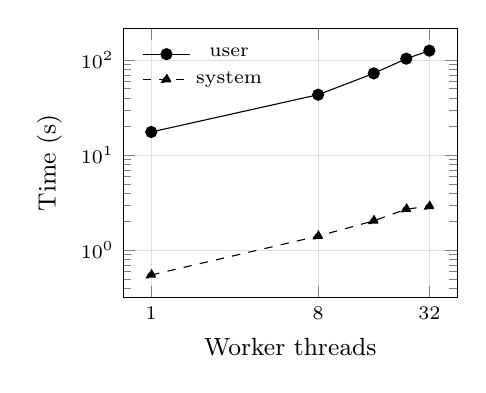
\begin{tikzpicture}
\begin{axis}[
    width=0.48\textwidth, height=5.0cm,
    xlabel={Worker threads}, ylabel={Time (s)},
    xmode=log, log basis x=2, xtick={1,8,32}, xticklabels={1,8,32},
    ymode=log, grid=major, grid style={gray!25},
    legend style={font=\scriptsize, at={(0.03,0.97)}, anchor=north west, draw=none, fill=none},
    label style={font=\small}, tick label style={font=\scriptsize},
]
% GENERATED by tools/dev/paper_tables.py -- do not edit.
% commit ca4a52b | measured on AMD EPYC 9174F 16-Core Processor, 503 GB RAM, Linux 6.8.0-138-generic | load at start 2.62/3.47 (1m/15m) | source: tools/sampling_cost_smoke.cpp under procstat.measure

\addplot[mark=*, black] coordinates {(1,17.55)(8,43.28)(16,72.58)(24,103.58)(32,125.83)};
\addlegendentry{user}
\addplot[mark=triangle*, black, dashed] coordinates {(1,0.55)(8,1.41)(16,2.04)(24,2.71)(32,2.90)};
\addlegendentry{system}

\end{axis}
\end{tikzpicture}
\caption{User and system time against worker count, for the runs of
Table~\ref{tab:t13-memory}: across a $\ThreadSweepFactor\times$ increase in workers, user time
grows $\UserTimeGrowth\times$ and system time, thirty to forty-five times smaller, grows
$\SysTimeGrowth\times$.}
\label{fig:scaling}
\end{figure}

\subsection{Parallel Efficiency by Rule Shape}
The amount of parallel work in a run depends on the rule. Table~\ref{tab:t12-shapes} measures two
rules at every thread count: a one-edge left-hand side, which matches by an index scan and expands
each state narrowly, and a two-edge left-hand side, which matches by a join and produces a wider
frontier. With both sized to seconds of single-threaded work, their efficiencies are within a few
points of each other at every thread count (the lower of the two is $\EffAtEight$ at eight threads
and $\EffAtSixteen$ at sixteen), and both still gain in wall time at thirty-two threads. The
decline is not thread start-up, since both single-threaded runs take seconds; it starts at the
thread count that first uses a second L3 domain (Section~\ref{sec:memory-scaling}).
Section~\ref{sec:lhs-space} measures the same size axis at four sizes and greater depths, together
with two other properties of the left-hand side.

\begin{table}[htbp]
\centering
\caption{Wall time and parallel efficiency by thread count for a one-edge and a
two-edge left-hand side.}
\label{tab:t12-shapes}
% GENERATED by tools/dev/paper_tables.py -- do not edit.
% commit e264560 | measured on AMD EPYC 9174F 16-Core Processor, 503 GB RAM, Linux 6.8.0-138-generic | load at start 3.05/4.04 (1m/15m) | source: tools/sampling_cost_smoke.cpp
{\footnotesize\setlength{\tabcolsep}{4pt}%
\resizebox{\ifdim\width>\linewidth\linewidth\else\width\fi}{!}{%
\begin{tabular}{rrrrr}
\toprule
Threads & \multicolumn{2}{c}{one-edge LHS} & \multicolumn{2}{c}{two-edge LHS} \\
 & ms & eff. & ms & eff. \\
\midrule
1 & 18076.0 & 1.00 & 12228.5 & 1.00 \\
2 & 9779.1 & 0.92 & 6746.5 & 0.91 \\
4 & 7034.7 & 0.64 & 4816.4 & 0.63 \\
8 & 5561.6 & 0.41 & 4156.2 & 0.37 \\
16 & 4606.0 & 0.25 & 3612.3 & 0.21 \\
24 & 4414.6 & 0.17 & 3522.3 & 0.14 \\
32 & 4097.0 & 0.14 & 3291.2 & 0.12 \\
\bottomrule
\end{tabular}
}}

\end{table}

\subsection{Left-Hand-Side Properties}
\label{sec:lhs-space}

A left-hand side has three independent properties, each of which changes the matching problem:

\begin{itemize}
\item \textbf{Size}: the number of edges to bind. Each edge adds a factor to the search and a
      constraint that prunes it.
\item \textbf{Arity}: the number of vertices per edge, which sets how much of the state one bound
      edge determines.
\item \textbf{Connectivity}: how the edges share vertices. A path shares one vertex between
      consecutive edges; a star shares one vertex among all of them; a ring has no end; and a
      left-hand side with components that share no vertex is matched as a cartesian product,
      quadratic in the state size for two components.
\end{itemize}

Figure~\ref{fig:time-corpus} gives the wall times of the sweep's ten timed workloads at every thread
count, each at the deepest depth whose single-threaded run fits the sweep's time budget, and
Figure~\ref{fig:lhs-scaling} gives the same measurements as parallel efficiency along each
property. Every curve in Figure~\ref{fig:time-corpus} falls through 32 threads, mostly below
sixteen: going from one thread to eight divides wall time by $2.3$ (the star) to $4.5$ (the
mixed-arity chain), and going from sixteen threads to 32 reduces it by a further $4.6$ to $23.7$
percent.

\begin{figure}[htbp]
\centering
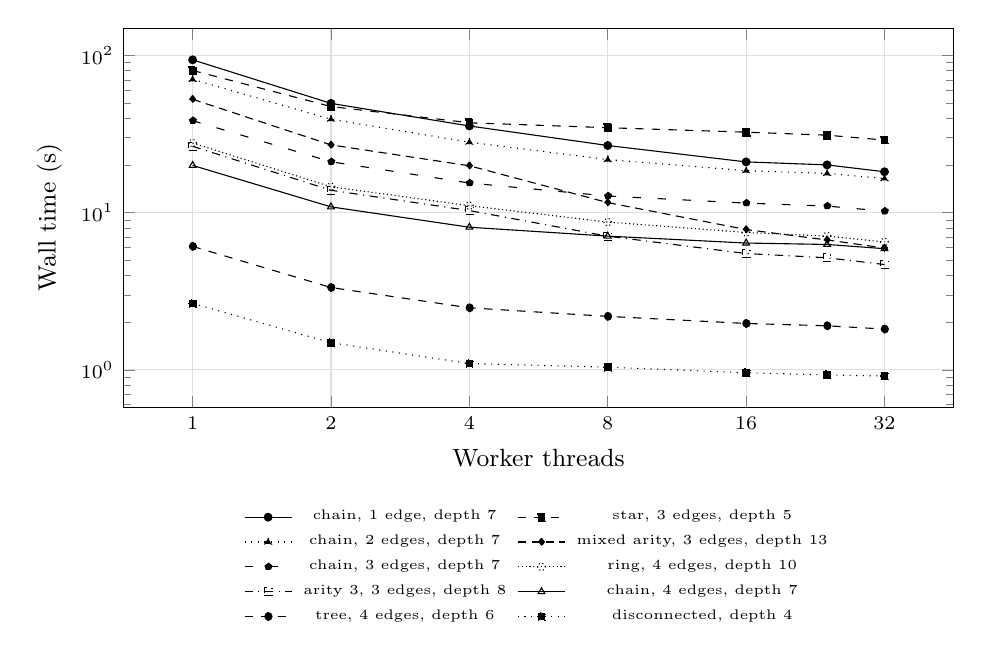
\begin{tikzpicture}
\begin{axis}[
    width=\linewidth, height=6.4cm,
    xlabel={Worker threads}, ylabel={Wall time (s)},
    xmode=log, log basis x=2, xtick={1,2,4,8,16,32}, xticklabels={1,2,4,8,16,32},
    ymode=log, grid=major, grid style={gray!25},
    legend style={font=\tiny, at={(0.5,-0.24)}, anchor=north, legend columns=2,
                  draw=none, fill=none, column sep=2pt, inner xsep=1pt},
    label style={font=\small}, tick label style={font=\scriptsize},
]
% GENERATED by tools/dev/paper_tables.py -- do not edit.
% commit 0ada228c | measured on AMD EPYC 9174F 16-Core Processor | table generated on Intel(R) Core(TM) i9-14900K, 31 GB RAM, Linux 5.15.167.4-microsoft-standard-WSL2 | source: tools/dev/rich_sweep.sh over tools/sampling_cost_smoke.cpp

\addplot[mark=*, black, solid, mark size=1.4pt] coordinates {(1,93.878)(2,49.606)(4,35.632)(8,26.764)(16,21.049)(24,20.145)(32,18.221)};
\addlegendentry{chain, 1 edge, depth 7}
\addplot[mark=square*, black, dashed, mark size=1.4pt] coordinates {(1,80.373)(2,47.377)(4,37.334)(8,34.735)(16,32.536)(24,31.135)(32,28.995)};
\addlegendentry{star, 3 edges, depth 5}
\addplot[mark=triangle*, black, dotted, mark size=1.4pt] coordinates {(1,70.547)(2,39.330)(4,28.093)(8,21.781)(16,18.513)(24,17.780)(32,16.494)};
\addlegendentry{chain, 2 edges, depth 7}
\addplot[mark=diamond*, black, densely dashed, mark size=1.4pt] coordinates {(1,52.686)(2,27.002)(4,19.892)(8,11.596)(16,7.813)(24,6.708)(32,5.962)};
\addlegendentry{mixed arity, 3 edges, depth 13}
\addplot[mark=pentagon*, black, loosely dashed, mark size=1.4pt] coordinates {(1,38.523)(2,21.099)(4,15.448)(8,12.769)(16,11.509)(24,11.022)(32,10.227)};
\addlegendentry{chain, 3 edges, depth 7}
\addplot[mark=o, black, densely dotted, mark size=1.4pt] coordinates {(1,27.754)(2,14.628)(4,11.082)(8,8.718)(16,7.483)(24,7.104)(32,6.515)};
\addlegendentry{ring, 4 edges, depth 10}
\addplot[mark=square, black, dashdotted, mark size=1.4pt] coordinates {(1,26.444)(2,13.890)(4,10.318)(8,7.086)(16,5.499)(24,5.167)(32,4.681)};
\addlegendentry{arity 3, 3 edges, depth 8}
\addplot[mark=triangle, black, solid, mark size=1.4pt] coordinates {(1,19.988)(2,10.892)(4,8.083)(8,7.096)(16,6.413)(24,6.280)(32,5.904)};
\addlegendentry{chain, 4 edges, depth 7}
\addplot[mark=*, black, dashed, mark size=1.4pt] coordinates {(1,6.105)(2,3.342)(4,2.482)(8,2.190)(16,1.974)(24,1.908)(32,1.818)};
\addlegendentry{tree, 4 edges, depth 6}
\addplot[mark=square*, black, dotted, mark size=1.4pt] coordinates {(1,2.648)(2,1.489)(4,1.097)(8,1.041)(16,0.958)(24,0.929)(32,0.914)};
\addlegendentry{disconnected, depth 4}

\end{axis}
\end{tikzpicture}
\caption{Wall time against worker count for the sweep's ten timed workloads, each at the depth its
legend entry states. Both axes are logarithmic; the legend lists the curves in descending order of
single-threaded time.}
\label{fig:time-corpus}
\end{figure}

The four chain sizes run at depth seven, so the size comparison is controlled. Single-threaded
wall time falls as the left-hand side grows: $93.9$, $70.5$, $38.5$ and $20.0$\,s for one to four
edges, following the state count at that depth ($18{,}636{,}561$ down to $1{,}831{,}446$;
Table~\ref{tab:t14-shape-space}). Efficiency at 32 threads falls in the same order: $0.161$,
$0.134$, $0.118$, $0.106$. Table~\ref{tab:t12-shapes} measures two different rules at different
depths, so its columns are not comparable with these.

At 32 threads, efficiency along the connectivity axis ranges from $0.087$ to $0.133$: ring $0.133$,
path $0.118$, branching tree $0.105$, disconnected $0.091$ and hub $0.087$. The disconnected shape
also suffers from cache traffic between L3 domains. At a fixed two threads, the disconnected
workload takes $976$\,ms when both threads share an L3 domain and $1494$\,ms when they do not,
against $1322$\,ms on one thread.

Arity gives the widest spread. With a three-edge left-hand side, efficiency at 32 threads is
$0.118$ at arity two, $0.177$ at arity three, and $0.276$, the highest in the sweep, with arities
alternating between two and three (at depths seven, eight and thirteen). In a path of arity three,
consecutive edges share two vertices, which fixes a match's orientation, so each state has a
narrower frontier and more of its children are duplicates.

\begin{figure}[htbp]
\centering
\begin{subfigure}{\linewidth}
\centering
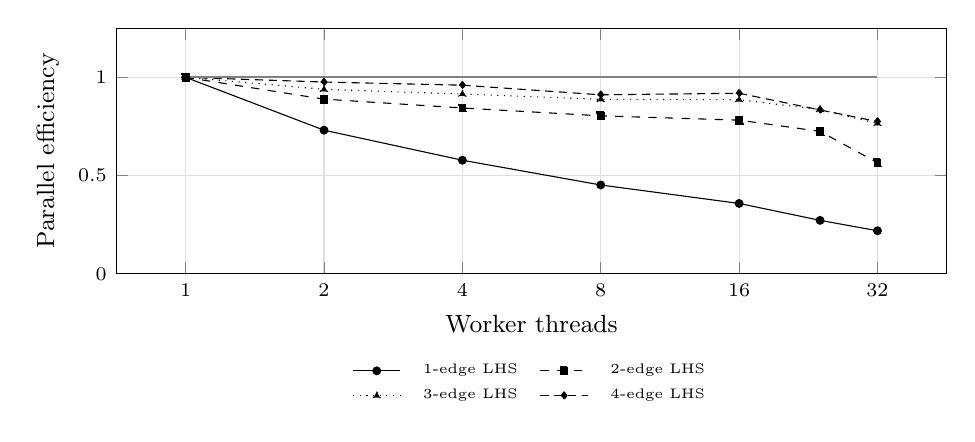
\begin{tikzpicture}
\begin{axis}[
    width=\linewidth, height=4.7cm,
    xlabel={Worker threads}, ylabel={Parallel efficiency},
    xmode=log, log basis x=2, xtick={1,2,4,8,16,32}, xticklabels={1,2,4,8,16,32},
    ymin=0, ymax=1.25, grid=major, grid style={gray!25},
    legend style={font=\tiny, at={(0.5,-0.32)}, anchor=north, legend columns=2,
                  draw=none, fill=none, column sep=6pt},
    label style={font=\small}, tick label style={font=\scriptsize},
]
% GENERATED by tools/dev/paper_tables.py -- do not edit.
% commit 61c409ca | measured on AMD EPYC 9174F 16-Core Processor | table generated on Intel(R) Core(TM) i9-14900K, 20 GB RAM, Linux 5.15.167.4-microsoft-standard-WSL2 | source: tools/dev/rich_sweep.sh over tools/sampling_cost_smoke.cpp

\addplot[mark=*, black, solid, mark size=1.4pt] coordinates {(1,1.000)(2,0.731)(4,0.578)(8,0.452)(16,0.358)(24,0.272)(32,0.219)};
\addlegendentry{1-edge LHS}
\addplot[mark=square*, black, dashed, mark size=1.4pt] coordinates {(1,1.000)(2,0.889)(4,0.844)(8,0.804)(16,0.782)(24,0.725)(32,0.565)};
\addlegendentry{2-edge LHS}
\addplot[mark=triangle*, black, dotted, mark size=1.4pt] coordinates {(1,1.000)(2,0.939)(4,0.915)(8,0.888)(16,0.886)(24,0.836)(32,0.765)};
\addlegendentry{3-edge LHS}
\addplot[mark=diamond*, black, densely dashed, mark size=1.4pt] coordinates {(1,1.000)(2,0.976)(4,0.960)(8,0.911)(16,0.919)(24,0.834)(32,0.775)};
\addlegendentry{4-edge LHS}
\addplot[gray, thick, no marks, forget plot] coordinates {(1,1)(32,1)};

\end{axis}
\end{tikzpicture}
\caption{Left-hand-side size: one to four edges, all binary chains.}
\end{subfigure}

\vspace{2mm}
\begin{subfigure}{\linewidth}
\centering
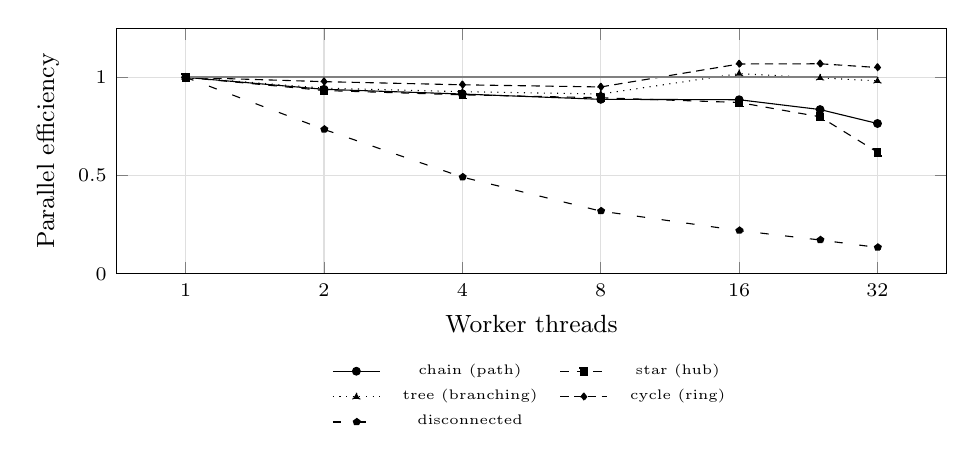
\begin{tikzpicture}
\begin{axis}[
    width=\linewidth, height=4.7cm,
    xlabel={Worker threads}, ylabel={Parallel efficiency},
    xmode=log, log basis x=2, xtick={1,2,4,8,16,32}, xticklabels={1,2,4,8,16,32},
    ymin=0, ymax=1.25, grid=major, grid style={gray!25},
    legend style={font=\tiny, at={(0.5,-0.32)}, anchor=north, legend columns=2,
                  draw=none, fill=none, column sep=6pt},
    label style={font=\small}, tick label style={font=\scriptsize},
]
% GENERATED by tools/dev/paper_tables.py -- do not edit.
% commit 61c409ca | measured on AMD EPYC 9174F 16-Core Processor | table generated on Intel(R) Core(TM) i9-14900K, 20 GB RAM, Linux 5.15.167.4-microsoft-standard-WSL2 | source: tools/dev/rich_sweep.sh over tools/sampling_cost_smoke.cpp

\addplot[mark=*, black, solid, mark size=1.4pt] coordinates {(1,1.000)(2,0.939)(4,0.915)(8,0.888)(16,0.886)(24,0.836)(32,0.765)};
\addlegendentry{chain (path)}
\addplot[mark=square*, black, dashed, mark size=1.4pt] coordinates {(1,1.000)(2,0.933)(4,0.911)(8,0.896)(16,0.872)(24,0.799)(32,0.619)};
\addlegendentry{star (hub)}
\addplot[mark=triangle*, black, dotted, mark size=1.4pt] coordinates {(1,1.000)(2,0.945)(4,0.927)(8,0.915)(16,1.019)(24,0.997)(32,0.982)};
\addlegendentry{tree (branching)}
\addplot[mark=diamond*, black, densely dashed, mark size=1.4pt] coordinates {(1,1.000)(2,0.978)(4,0.962)(8,0.951)(16,1.068)(24,1.069)(32,1.050)};
\addlegendentry{cycle (ring)}
\addplot[mark=pentagon*, black, loosely dashed, mark size=1.4pt] coordinates {(1,1.000)(2,0.735)(4,0.492)(8,0.319)(16,0.220)(24,0.172)(32,0.134)};
\addlegendentry{disconnected}
\addplot[gray, thick, no marks, forget plot] coordinates {(1,1)(32,1)};

\end{axis}
\end{tikzpicture}
\caption{Connectivity at comparable size: path, hub, branching tree, ring, two disjoint
components.}
\end{subfigure}

\vspace{2mm}
\begin{subfigure}{\linewidth}
\centering
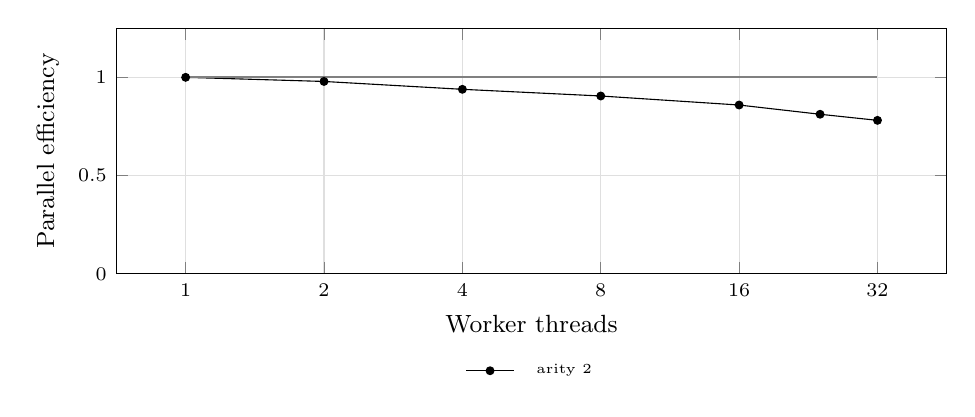
\begin{tikzpicture}
\begin{axis}[
    width=\linewidth, height=4.7cm,
    xlabel={Worker threads}, ylabel={Parallel efficiency},
    xmode=log, log basis x=2, xtick={1,2,4,8,16,32}, xticklabels={1,2,4,8,16,32},
    ymin=0, ymax=1.25, grid=major, grid style={gray!25},
    legend style={font=\tiny, at={(0.5,-0.32)}, anchor=north, legend columns=2,
                  draw=none, fill=none, column sep=6pt},
    label style={font=\small}, tick label style={font=\scriptsize},
]
% GENERATED by tools/dev/paper_tables.py -- do not edit.
% commit 97526beb | measured on AMD EPYC 9174F 16-Core Processor | table generated on Intel(R) Core(TM) i9-14900K, 20 GB RAM, Linux 5.15.167.4-microsoft-standard-WSL2 | source: tools/dev/rich_sweep.sh over tools/sampling_cost_smoke.cpp

\addplot[mark=*, black, solid, mark size=1.4pt] coordinates {(1,1.000)(2,0.979)(4,0.939)(8,0.905)(16,0.859)(24,0.812)(32,0.781)};
\addlegendentry{arity 2}
\addplot[gray, thick, no marks, forget plot] coordinates {(1,1)(32,1)};

\end{axis}
\end{tikzpicture}
\caption{Edge arity at a fixed three-edge left-hand side.}
\end{subfigure}
\caption{Parallel efficiency along the three properties of a left-hand side. Each curve is
normalized by its own single-threaded time on the same binary, workload and canonicalization
mode; the grey line $y=1$ is ideal scaling.}
\label{fig:lhs-scaling}
\end{figure}

\subsection{Evolution Depth and Relation Sizes}
\label{sec:shape-space}

Each shape is evolved one depth at a time until a single run exceeds the collection budget, so the
right-hand end of each curve in Figure~\ref{fig:shape-space} is the deepest depth that shape
reached within the budget. Runs that filled a container are excluded, because such a run returns
a truncated graph: one shape returns the same $2{,}097{,}149$ states when asked for depth 9, 10 or
11. Of the $192$ collected points, $41$ are excluded for this reason.

States and relation sizes vary independently. At around $300$k states the two-component shape has
$3.2$M branchial edges while a mixed-arity chain of similar size has none, and across the sweep the
branchial count ranges from zero to $58.8$M. Branchial edges connect pairs of events from the same
state that share a consumed edge, so their number depends on how many matches overlap rather than
on how many states exist, and a shape's position on the right panel of
Figure~\ref{fig:shape-space} is a property of its rule. Table~\ref{tab:t14-shape-space} gives the
deepest point each shape reached within the budget without filling a container, so depths differ
between rows. \texttt{chain2a3} and \texttt{chain2a4} have identical counts because in a path of
arity three or more consecutive edges already share enough vertices to fix a match's orientation,
so the two searches are the same.

A one-edge left-hand side produces no branchial edges at any depth, because two matches of a
single-edge pattern cannot share an edge. Every shape with two or more edges produces them.

\begin{figure}[htbp]
\centering
\begin{subfigure}{\linewidth}
\centering
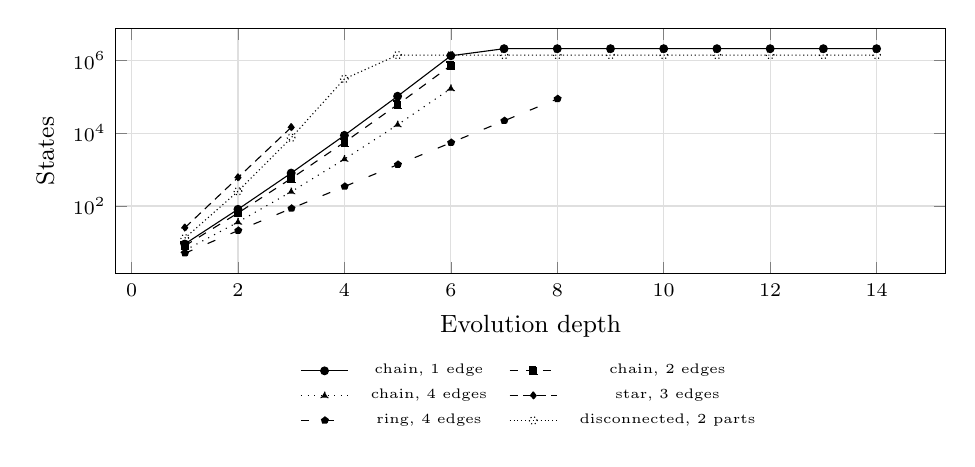
\begin{tikzpicture}
\begin{axis}[
    width=\linewidth, height=4.7cm,
    xlabel={Evolution depth}, ylabel={States},
    ymode=log, log basis y=10, grid=major, grid style={gray!25},
    legend style={font=\tiny, at={(0.5,-0.32)}, anchor=north, legend columns=2,
                  draw=none, fill=none, column sep=6pt},
    label style={font=\small}, tick label style={font=\scriptsize},
]
% GENERATED by tools/dev/paper_tables.py -- do not edit.
% commit 78c2f411 | measured on Intel(R) Core(TM) i9-14900K, 20 GB RAM, Linux 5.15.167.4-microsoft-standard-WSL2 | source: tools/dev/rich_sweep.sh over tools/sampling_cost_smoke.cpp

\addplot[mark=*, black, solid, mark size=1.4pt] coordinates {(1,9)(2,81)(3,801)(4,8721)(5,103761)(6,1339281)(7,2097148)(8,2097148)(9,2097149)(10,2097149)(11,2097149)(12,2097148)(13,2097148)(14,2097149)};
\addlegendentry{chain, 1 edge}
\addplot[mark=square*, black, dashed, mark size=1.4pt] coordinates {(1,8)(2,64)(3,568)(4,5608)(5,61048)(6,726328)};
\addlegendentry{chain, 2 edges}
\addplot[mark=triangle*, black, dotted, mark size=1.4pt] coordinates {(1,6)(2,36)(3,246)(4,1926)(5,17046)(6,168246)};
\addlegendentry{chain, 4 edges}
\addplot[mark=diamond*, black, densely dashed, mark size=1.4pt] coordinates {(1,25)(2,601)(3,14425)};
\addlegendentry{star, 3 edges}
\addplot[mark=pentagon*, black, loosely dashed, mark size=1.4pt] coordinates {(1,5)(2,21)(3,85)(4,341)(5,1365)(6,5461)(7,21845)(8,87381)};
\addlegendentry{ring, 4 edges}
\addplot[mark=o, black, densely dotted, mark size=1.4pt] coordinates {(1,13)(2,253)(3,7453)(4,309853)(5,1398101)(6,1398101)(7,1398100)(8,1398101)(9,1398101)(10,1398101)(11,1398101)(12,1398101)(13,1398101)(14,1398100)};
\addlegendentry{disconnected, 2 parts}

\end{axis}
\end{tikzpicture}
\caption{States against evolution depth, logarithmic in states.}
\end{subfigure}

\vspace{2mm}
\begin{subfigure}{\linewidth}
\centering
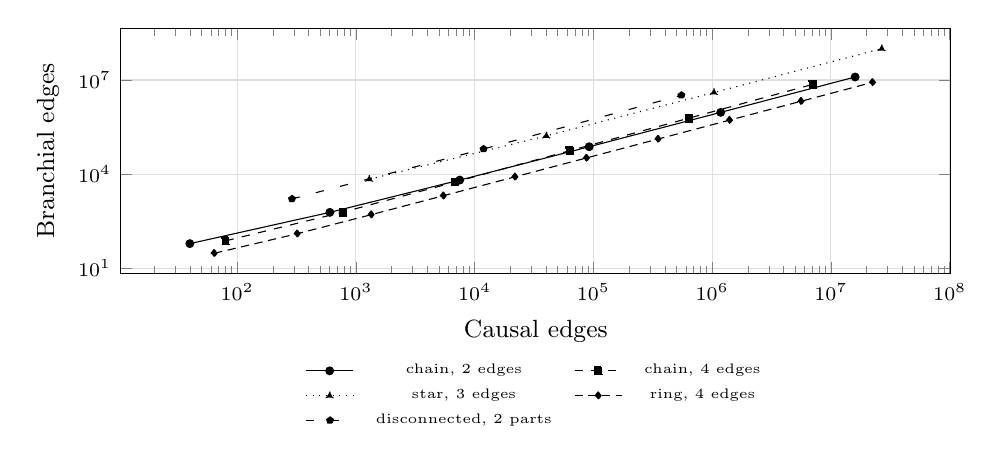
\begin{tikzpicture}
\begin{axis}[
    width=\linewidth, height=4.7cm,
    xlabel={Causal edges}, ylabel={Branchial edges},
    xmode=log, log basis x=10, ymode=log, log basis y=10,
    grid=major, grid style={gray!25},
    legend style={font=\tiny, at={(0.5,-0.32)}, anchor=north, legend columns=2,
                  draw=none, fill=none, column sep=6pt},
    label style={font=\small}, tick label style={font=\scriptsize},
]
% GENERATED by tools/dev/paper_tables.py -- do not edit.
% commit 9fb10394 | measured on AMD EPYC 9174F 16-Core Processor | table generated on Intel(R) Core(TM) i9-14900K, 31 GB RAM, Linux 5.15.167.4-microsoft-standard-WSL2 | source: tools/dev/rich_sweep.sh over tools/sampling_cost_smoke.cpp

\addplot[mark=*, black, solid, mark size=1.4pt] coordinates {(40,61)(604,606)(7492,6463)(92164,74609)(1180804,930055)(15998404,12470527)};
\addlegendentry{chain, 2 edges}
\addplot[mark=square*, black, dashed, mark size=1.4pt] coordinates {(80,75)(780,618)(6828,5588)(63276,55760)(639276,610019)(7054476,7264602)};
\addlegendentry{chain, 4 edges}
\addplot[mark=triangle*, black, dotted, mark size=1.4pt] coordinates {(1296,6900)(40176,165876)(1035504,3994260)(26779248,99436884)};
\addlegendentry{star, 3 edges}
\addplot[mark=diamond*, black, densely dashed, mark size=1.4pt] coordinates {(64,30)(320,126)(1344,510)(5440,2046)(21824,8190)(87360,32766)(349504,131070)(1398080,524286)(5592384,2097150)(22369600,8388606)};
\addlegendentry{ring, 4 edges}
\addplot[mark=pentagon*, black, loosely dashed, mark size=1.4pt] coordinates {(288,1614)(11808,62814)(547488,3238014)};
\addlegendentry{disconnected, 2 parts}

\end{axis}
\end{tikzpicture}
\caption{Branchial edges against causal edges, both logarithmic; each point is one
(shape, depth) run.}
\end{subfigure}
\caption{The state space and its relations, by left-hand-side shape.}
\label{fig:shape-space}
\end{figure}

\begin{table}[htbp]
\centering
\caption{The deepest point reached by each left-hand-side shape: \texttt{Shape}
the connectivity, \texttt{Arity} the vertices per edge, \texttt{LHS} the pattern's edge count;
the remaining columns are the sizes of the three objects the run built.}
\label{tab:t14-shape-space}
% GENERATED by tools/dev/paper_tables.py -- do not edit.
% commit 97526beb | measured on AMD EPYC 9174F 16-Core Processor | table generated on Intel(R) Core(TM) i9-14900K, 20 GB RAM, Linux 5.15.167.4-microsoft-standard-WSL2 | source: tools/dev/rich_sweep.sh over tools/sampling_cost_smoke.cpp
{\footnotesize\setlength{\tabcolsep}{4pt}%
\resizebox{\ifdim\width>\linewidth\linewidth\else\width\fi}{!}{%
\begin{tabular}{lrrrrrrr}
\toprule
Rule & Shape & Arity & LHS & Depth & States & Causal & Branchial \\
\midrule
\texttt{chain1a2} & chain & 2 & 1 & 6 & 1,339,281 & 850,896 & 0 \\
\texttt{growth} & chain & 2 & 1 & 10 & 4,037,914 & 4,037,912 & 0 \\
\texttt{chain2a2} & chain & 2 & 2 & 5 & 61,048 & 92,164 & 74,609 \\
\texttt{pair} & chain & 2 & 2 & 7 & 204,556 & 393,788 & 181,439 \\
\texttt{chain2a3} & chain & 3 & 2 & 5 & 19,608 & 26,732 & 16,806 \\
\texttt{chain2a4} & chain & 4 & 2 & 5 & 19,608 & 26,732 & 16,806 \\
\texttt{chain3a2} & chain & 2 & 3 & 5 & 33,649 & 87,920 & 81,725 \\
\texttt{triple} & chain & 2 & 3 & 6 & 23,116 & 66,980 & 37,362 \\
\texttt{chain3a3} & chain & 3 & 3 & 5 & 9,331 & 23,612 & 13,995 \\
\texttt{chain4a2} & chain & 2 & 4 & 5 & 17,046 & 63,276 & 55,760 \\
\texttt{quad} & chain & 2 & 4 & 6 & 23,116 & 90,092 & 51,609 \\
\texttt{cycle3a2} & cycle & 2 & 3 & 9 & 29,524 & 88,560 & 29,523 \\
\texttt{cycle4a2} & cycle & 2 & 4 & 7 & 21,845 & 87,360 & 32,766 \\
\texttt{disc2a2} & disc & 2 & 2 & 4 & 309,853 & 547,488 & 3,238,014 \\
\texttt{disc} & disc & 2 & 2 & 4 & 309,853 & 547,488 & 3,238,014 \\
\texttt{disc3a2} & disc & 2 & 3 & 4 & 1,045,591 & 3,136,752 & 58,835,751 \\
\texttt{mixed2} & mixed & 2 & 2 & 8 & 87,381 & 148,520 & 0 \\
\texttt{mixed3} & mixed & 2 & 3 & 9 & 29,524 & 85,978 & 19,682 \\
\texttt{mixed4} & mixed & 2 & 4 & 9 & 29,524 & 115,976 & 19,682 \\
\texttt{star2a2} & star & 2 & 2 & 4 & 26,293 & 45,792 & 108,378 \\
\texttt{star3a2} & star & 2 & 3 & 3 & 14,425 & 40,176 & 165,876 \\
\texttt{star4a2} & star & 2 & 4 & 3 & 14,425 & 57,600 & 165,876 \\
\texttt{tree3a2} & tree & 2 & 3 & 5 & 34,599 & 89,552 & 82,480 \\
\texttt{tree4a2} & tree & 2 & 4 & 5 & 40,655 & 148,628 & 179,283 \\
\bottomrule
\end{tabular}
}}

\end{table}

\subsection{Memory Behavior under Thread Scaling}
\label{sec:memory-scaling}
Falling efficiency at high thread counts could come from contention on the shared structures or
from the cost of acquiring memory. Table~\ref{tab:t13-memory} gives \texttt{getrusage} figures for
a workload of eighteen seconds of single-threaded work. Across a $\ThreadSweepFactor\times$
increase in workers, user time grows $\UserTimeGrowth\times$ and system time
$\SysTimeGrowth\times$, reaching $2.9$\,s of $128.7$\,s of CPU time at 32 workers, so the extra
time is in user code. Peak
resident set grows by a quarter and minor faults eleven-fold, and system time, which follows the
faults as each worker draws its own arena blocks, stays small, so memory acquisition is not the
cause. The instruction count is flat across the sweep (below), so spinning is not the cause either.

Hardware counters identify the cause. On the Wolfram rule at depth seven, executed instructions
are $14.5$G at one thread and $15.8$G at 32, while cycles double, so instructions per cycle fall
from $1.44$ to $0.69$. The counter that grows is demand fills served from another L3 domain's cache
(AMD \texttt{ls\_dmnd\_fills\_from\_sys.near\_cache}): $47$k at one thread and $10.6$M at 32. Fills
from DRAM and from the local cache hierarchy stay flat. Two experiments rule out the concurrent
structures as the source. Limiting the shared table's probe length from $32$ to $4$ leaves the fill
count unchanged and makes the run slower. A thread-private filter that removes $80\%$ of the
repeated inserts into the shared set lowers the set's share of the fills from $36\%$ to $12\%$
without changing the total or the wall time; the fills move to neighboring code. The traffic comes
from the evolution itself: about twelve cross-domain fills per object created, because a state
created on one core complex is read by workers on others, and this part has eight L3 domains.

The effect is visible in wall time when a run first uses a second L3 domain. Sweeping every worker
count from one to thirty-two, with workers pinned one per physical core in order, on a part whose
L3 domains hold two cores each: wall time falls from one worker to two, rises from two to three
on every large workload (\texttt{wpp} by $12.7\%$, \texttt{wolfram24} by $20.4\%$,
\texttt{wolftri} by $12.8\%$, \texttt{multirule} by $36.1\%$), and falls again from four onward.
The third worker is the first in a second domain. Placing that worker on an SMT sibling in the
first domain removes the rise (\texttt{wpp} $347$ to $258$\,ms at three workers, below the
two-worker time), and the rise moves to the fourth worker, which opens the second domain. Filling
each domain's two cores and their two SMT siblings before using the next domain is faster at every
count measured, including sixteen workers (\texttt{wpp} $197$ to $182$\,ms, \texttt{wolfram24}
$36.3$ to $33.3$\,ms, \texttt{multirule} $34.7$ to $25.7$\,ms), although it uses half as many
physical cores at sixteen. This packed placement is the engine's default and was used for every
table in this section. Under it the rise moves to the fifth worker, the first in a second domain:
\texttt{wpp} takes $216$\,ms at four workers, $247$ at five, $234$ at six and $205$ at eight, and
later domains add at most $2.3\%$ at any count from one to thirty-two. At powers of two the curve
falls monotonically. These measurements depend on the host: on a part with larger L3 domains the
second domain opens at a higher worker count.

\begin{table}[htbp]
\centering
\caption{User and system time, peak resident set and minor page faults against
thread count, from \texttt{getrusage}.}
\label{tab:t13-memory}
% GENERATED by tools/dev/paper_tables.py -- do not edit.
% commit f53a191 | measured on AMD EPYC 9174F 16-Core Processor, 503 GB RAM, Linux 6.8.0-138-generic | load at start 3.10/1.73 (1m/15m) | source: tools/sampling_cost_smoke.cpp under procstat.measure
{\footnotesize\setlength{\tabcolsep}{4pt}%
\resizebox{\ifdim\width>\linewidth\linewidth\else\width\fi}{!}{%
\begin{tabular}{rrrrrr}
\toprule
Threads & Wall s & User s & System s & Peak RSS MB & Minor faults \\
\midrule
1 & 3.09 & 2.73 & 0.35 & 624 & 160\,040 \\
8 & 1.00 & 6.36 & 0.80 & 1184 & 311\,547 \\
16 & 0.80 & 8.46 & 1.51 & 1816 & 483\,330 \\
24 & 0.77 & 10.60 & 2.39 & 2377 & 633\,698 \\
32 & 0.82 & 12.73 & 3.25 & 2865 & 768\,659 \\
\bottomrule
\end{tabular}
}}

\end{table}

\subsection{Device Saturation}
The resident kernel is launched with a fixed number of blocks per streaming multiprocessor, so that
number is a tuning parameter. Wall time falls as blocks are added until eight per SM, the default,
and sixteen per SM is within measurement variation of eight (Table~\ref{tab:t11-saturation}). The
last column, the driver's peak SM-busy reading, reports whether the multiprocessors were busy, not
how many warps were resident; it reads $100\%$ at every point.

\begin{table}[htbp]
\centering
\caption{Wall time and peak SM-busy against blocks per streaming multiprocessor.}
\label{tab:t11-saturation}
% GENERATED by tools/dev/paper_tables.py -- do not edit.
% commit 769b12ba | Intel(R) Core(TM) i9-14900K, 20 GB RAM, Linux 5.15.167.4-microsoft-standard-WSL2 | source: tools/bench_gpu_evolve.cpp (mode 2) + driver utilisation sampling
\resizebox{\ifdim\width>\linewidth\linewidth\else\width\fi}{!}{%
\begin{tabular}{rrrrl}
\toprule
Blocks per SM & Blocks & Median ms & vs.\ 1 per SM & Peak SM-busy \\
\midrule
1 & 128 & 6.15 & 1.00$\times$ & 91\% \\
2 & 256 & 6.13 & 1.00$\times$ & 92\% \\
4 & 512 & 5.40 & 1.14$\times$ & 98\% \\
8 & 1024 & 5.91 & 1.04$\times$ & 86\% \\
16 & 2048 & 5.75 & 1.07$\times$ & 97\% \\
\bottomrule
\end{tabular}
}

\end{table}

\subsection{Occupancy and Lane Efficiency}
\label{sec:device-bounds}

Table~\ref{tab:device-occupancy} gives occupancy, throughput and active lanes per warp for the
resident kernel on every corpus workload, from hardware counters under Nsight Compute.

\textbf{Occupancy.} \texttt{cuobjdump -res-usage} on the linked binary reports that
\texttt{k\_persistent\_evolve} uses 255 registers per thread, the architectural maximum. At 32
threads per block a block reserves $8{,}160$ registers, and an sm\_89 multiprocessor has
$65{,}536$, so eight blocks fit: 256 resident threads against a maximum of $1{,}536$, an occupancy
of $16.7\%$. The launch grid is also eight blocks per multiprocessor, so the two limits coincide.
The measured occupancy is $14.1\%$ to $17.3\%$ on every corpus workload, over kernel durations that
differ by a factor of seven hundred. Limiting the kernel to 128 registers halves the register
allocation and leaves occupancy unchanged, so the grid, not the register count, sets it. Doubling
the grid under that limit doubles residency and makes the kernel slower, increasingly so as the grid
grows, because the added warps compete for the shared work queues without adding independent work.

\textbf{Active lanes.} The canonicalization phase runs on the whole warp: refinement's loops are
spread across the lanes, and the search's serial steps (individualization, orbit closure, backtracking)
run on one lane while the others wait at warp barriers. Publication, signature, quotient and
deduplication steps run on one lane. On \texttt{wpp} at depth six the kernel averages $3.5$ active
lanes per warp out of $32$. Per-block \texttt{clock64} timing shows that, on the workloads with
enough work to measure, canonicalization takes most block cycles, rewriting a few percent and
matching under two.

\textbf{Throughput.} No hardware unit is near its limit. On \texttt{wpp} at depth six SM
throughput is $9.7\%$ of peak, memory throughput $24.3\%$ and DRAM $11.6\%$; across the corpus the
maxima are $12.6\%$, $33.8\%$ and $16.1\%$. Atomic operations, which the work queues use, are
served by L2, whose throughput is included in the memory figure.

On the large workloads the device is therefore limited by the serial steps of the IR search, in
which each step depends on the one before, and not by bandwidth, queue contention or occupancy. A
separate measurement records no time spent waiting for unpublished work.

\textbf{Workloads with few classes.} The workloads with few states behave differently. With causal
recording on, \texttt{cycle4} and \texttt{multirule} reconstruct causal relations far larger than
their state counts and still leave the device idle most of the time, with SM throughput of $2.2\%$
and DRAM $0.01\%$ on \texttt{cycle4}, and $9.8$ and $10.4$ active lanes. The kernel takes four
times longer on \texttt{multirule}'s $49$ states than on \texttt{wolfram24}'s $9{,}820$. At depth
six \texttt{cycle4} replays $68{,}185$ instances over $40$ classes and is slower than the host,
while \texttt{wolfram24} replays $86{,}086$ instances over $9{,}820$ classes and is faster. The
instance counts are similar and the class counts differ by a factor of 250. The replay walks each
class's instances on one worker, so a run with forty classes has forty workers' worth of parallel
work however many instances it holds. \texttt{cycle4} starts from an initial state with many
automorphisms, which collapses its states into few classes.

\textbf{Causal recording.} The measurements above run with causal recording off. With it on, the
device and host reconstruct the same causal relation on all eight corpus workloads the device
supports, at depth six: the same number of distinct pairs and the same number after transitive
reduction. On the densest available workload, a three-edge disconnected left-hand side at depth
three, both give $1{,}661{,}760$ causal pairs and $970{,}560$ after reduction. The two engines
share only the replay core, with separate schedulers, memory layouts and queues. Both store the
relation unreduced and reduce it when it is read, using one shared reduction; a finite DAG has one
transitive reduction, so the result does not depend on the order in which pairs arrive. The
reduction is computed once per source event, since every edge leaving an event shares the set
reachable from it in two or more steps, and when event identifiers increase along every causal
edge the search stops at the source's largest target. Branchial pairs are not stored: both engines
derive them from the applications when they are read.

\textbf{Host traffic.} Across every evolution traced, no copy, allocation or memset runs while the
resident kernel runs, including twenty-four consecutive evolutions with the reconstruction on. Each
evolution is preceded and followed by runtime allocation, copy and fill calls, in equal numbers, so
a session pays this cost on every call, and a single deep run pays it once.

When raw events are not requested, the replay does not run (Section~\ref{sec:quotient}). With the
replay on, \texttt{multirule} and \texttt{cycle4} do not complete depth seven; without it both
complete, with the same state and event counts.

\begin{table}[htbp]
\centering
\caption{\textbf{Resident-kernel occupancy, throughput and active lanes across the corpus},
from hardware counters under NVIDIA Nsight Compute: means over the profiled launches of the
resident kernel. Durations are the profiler's, which serializes execution and fixes clocks, and
are not comparable with the wall times of Table~\ref{tab:t7b-gpu-corpus}.}
\label{tab:device-occupancy}
\resizebox{\ifdim\width>\linewidth\linewidth\else\width\fi}{!}{%
% GENERATED by tools/dev/paper_tables.py -- do not edit.
% commit e264560a | measured on AMD EPYC 9174F 16-Core Processor, NVIDIA GeForce RTX 4090 | table generated on Intel(R) Core(TM) i9-14900K, 31 GB RAM, Linux 5.15.167.4-microsoft-standard-WSL2 | source: Nsight Compute over tools/bench_gpu_evolve.cpp (mode 2)
{\footnotesize\setlength{\tabcolsep}{4pt}%
\resizebox{\ifdim\width>\linewidth\linewidth\else\width\fi}{!}{%
\begin{tabular}{lrrrrrrrr}
\toprule
Workload & Depth & Launches & Duration (\textmu s) & SM \% & Mem.\ \% & DRAM \% & Lanes/warp & Occ.\ \% \\
\midrule
\texttt{disc2x2} & 6 & 7 & 178994.3 & 3.88 & 3.95 & 0.17 & 6.05 & 16.84 \\
\texttt{multirule} & 6 & 5 & 113454.0 & 2.24 & 2.30 & 0.02 & 10.41 & 17.25 \\
\texttt{growshrink3} & 6 & 12 & 81015.0 & 10.86 & 33.27 & 16.08 & 3.14 & 16.99 \\
\texttt{cycle4} & 6 & 3 & 73393.3 & 2.23 & 2.72 & 0.01 & 9.84 & 16.39 \\
\texttt{multiroot} & 6 & 3 & 13420.0 & 2.38 & 2.43 & 0.04 & 8.87 & 15.54 \\
\texttt{wolfram24} & 6 & 3 & 9086.7 & 12.59 & 33.75 & 12.88 & 2.71 & 16.41 \\
\texttt{wpp} & 6 & 3 & 3900.0 & 9.65 & 24.25 & 11.57 & 3.45 & 16.71 \\
\texttt{binary} & 6 & 3 & 2676.7 & 2.20 & 2.22 & 0.03 & 11.17 & 16.77 \\
\texttt{arity3} & 6 & 3 & 2106.7 & 2.20 & 2.17 & 0.03 & 11.59 & 16.42 \\
\texttt{triangle} & 6 & 3 & 263.8 & 2.60 & 2.95 & 0.21 & 11.59 & 16.28 \\
\bottomrule
\end{tabular}
}}
}
\end{table}

\subsection{Ablation}
Match forwarding is the one run-time switch that changes speed without changing the answer. The
state and event identity modes change which answer is computed, so a time ratio between them
compares different computations; Section~\ref{sec:event-canon} reports how their results differ,
and Table~\ref{tab:t6-quotient} reports quotient exploration. The static analysis of
Section~\ref{sec:static-analysis} turns forwarding on or off per rule set. Table~\ref{tab:t9-ablation}
gives best-of-$N$ wall times for both settings. On the one-edge left-hand side (depth eight) the
analysis turns forwarding off, and forwarding on is $1.16\times$ slower. On the two-edge left-hand
side (depth six) it turns forwarding on, and forwarding on is $1.10\times$ slower than off, a
difference within the run-to-run variation of runs that short on this machine. Both settings give
the same state and event counts on both workloads.

\begin{table}[htbp]
\centering
\caption{Match forwarding on and off: one-edge left-hand side at depth eight, two-edge at depth
six. Best-of-$N$ wall times; both settings give identical state and event counts.}
\label{tab:t9-ablation}
% GENERATED by tools/dev/paper_tables.py -- do not edit.
% commit e0cdb45f | Intel(R) Core(TM) i9-14900K, 20 GB RAM, Linux 5.15.167.4-microsoft-standard-WSL2 | source: tools/sampling_cost_smoke.cpp
\resizebox{\ifdim\width>\linewidth\linewidth\else\width\fi}{!}{%
\begin{tabular}{lllrlrl}
\toprule
Contribution & Arm A & A ms & Arm B & B ms & Ratio & Same answer \\
\midrule
Match forwarding, one-edge LHS & on & 116.9 & decided off & 94.5 & 1.24 & yes \\
Match forwarding, two-edge LHS & off & 239.9 & decided on & 157.9 & 1.52 & yes \\
State canonicalization & Full (exact) & 158.4 & Automatic (hash) & 168.8 & 0.94 & yes \\
\bottomrule
\end{tabular}
}

\end{table}

\subsection{Instruction Profile}
\label{sec:instruction-profile}

Executed instruction counts are deterministic for a single-threaded run and unaffected by other
load, so they attribute time to parts of the engine. Table~\ref{tab:t15-instructions}
comes from one \texttt{callgrind} run of a single-threaded depth-six evolution of the Wolfram rule
under quotient exploration with the raw relations reconstructed, the CPU benchmark's default
configuration. The quotient reconstruction ($\InstrShareRecon\%$) and canonicalization
($\InstrShareCanon\%$) are the two largest parts and are close; the concurrent sets and maps
($\InstrShareSets\%$) and libc's copies, fills and heap calls ($\InstrShareLibc\%$) follow; matching,
its join and the rewrite together are $\InstrShareMatch\%$. The unattributed $\InstrUnattributedPct\%$
is functions below the reporting threshold and code not assigned to a group.

\begin{table}[htbp]
\centering
\caption{Executed instructions by component: a single-threaded depth-six
evolution of the Wolfram rule under quotient exploration with reconstruction, under
\texttt{callgrind}, grouped by the algorithm each function belongs to. The per-function profile
covers $\InstrFlatCoverage\%$ of the program total; the rest is below the annotator's reporting
threshold. The benchmark-harness row is the corpus set-up the benchmark performs before the
evolution.}
\label{tab:t15-instructions}
% GENERATED by tools/dev/paper_tables.py -- do not edit.
% commit 61c409ca | measured on AMD EPYC 9174F 16-Core Processor | table generated on Intel(R) Core(TM) i9-14900K, 20 GB RAM, Linux 5.15.167.4-microsoft-standard-WSL2 | source: tools/dev/remote_session.sh attrib phase, callgrind over tools/bench_cpu_evolve
{\footnotesize\setlength{\tabcolsep}{4pt}%
\resizebox{\ifdim\width>\linewidth\linewidth\else\width\fi}{!}{%
\begin{tabular}{lrr}
\toprule
Component & Instructions & Share \\
\midrule
Match expansion and join & 117,653,606 & 24.7\% \\
Canonicalization (IR) & 79,592,324 & 16.7\% \\
Dedup sets and maps & 71,807,564 & 15.1\% \\
Arena allocation & 38,097,485 & 8.0\% \\
Hypergraph storage & 24,250,782 & 5.1\% \\
Causal and branchial & 728,120 & 0.2\% \\
Job system and work stealing & 366,201 & 0.1\% \\
\midrule
Unattributed & 139,143,506 & 29.2\% \\
\midrule
\textbf{Total} & 476,371,312 & 99.0\% \\
\bottomrule
\end{tabular}
}}

\end{table}

\paragraph{Cost per unit of work.} Each phase's instruction count divided by the number of items it
produces, from the same run: $\InstrIrCalls$ canonicalization calls over $\InstrRaw$ raw states,
$\InstrEvents$ reconstructed events, $\InstrSetInserts$ claim-set inserts and $\InstrCaptured$
applied matches. Canonicalization costs $\InstrIrPerCanonCall$ instructions per call on states of
two to fourteen edges. The search goes past its first node on $\InstrIrSearched$ of the
$\InstrIrCalls$ calls, so most calls cost one refinement to a stable partition, a few thousand
instructions at this size; the measured cost is several times that, with $\InstrCanonRefinePct\%$
of the phase in the refinement loop, $\InstrCanonHashPct\%$ in per-call set-up and the invariant
hash, and $\InstrCanonOrbitsPct\%$ in the orbit computation that quotient event identity needs.
Reconstruction costs $\InstrIrPerReconEvent$ instructions per event, against a minimum of one
identity claim, one producer lookup per consumed edge and one producer record per produced edge, a
few hundred instructions for a rule with two inputs and four outputs; the rest is in the
per-instance replay (\texttt{qr\_apply}) and in \texttt{register\_quotient\_transition}'s vector
operations. The claim sets cost $\InstrIrPerSetInsert$ instructions per insert against a minimum of
one hash, one probe and one exchange, about fifty; $\InstrSetRepeatPct\%$ of inserts offer a key
already present. Matching, the join and the rewrite cost $\InstrIrPerAppliedMatch$ instructions per
applied match, including building the match record and the child state. Every host phase costs more
than twice its minimum. The libc share is mostly the benchmark's own set-up, inlined into
\texttt{main} by link-time optimization, and the construction of rule objects.

\subsection{Event Identity}
Table~\ref{tab:event-canon} evolves each workload once, single-threaded in the exact state mode,
and counts distinct events under each of the three conventions of Section~\ref{sec:event-canon}:
by endpoint states, by consumed and produced edges, and by distinct applications. Each convention
refines the one before, so the counts do not decrease from left to right, and they differ on most
workloads: on \texttt{binary-growth} they are $5$, $8$ and $9$. Every other event count in this
paper counts distinct applications.

\begin{table}[htbp]
\centering
\caption{Distinct events per identity convention on each corpus workload.}
\label{tab:event-canon}
% GENERATED by tools/dev/paper_tables.py -- do not edit.
% commit eb8a742 | measured on AMD EPYC 9174F 16-Core Processor, 503 GB RAM, Linux 6.8.0-138-generic | load at start 1.04/1.78 (1m/15m) | source: tools/mode_matrix_probe.cpp
{\footnotesize\setlength{\tabcolsep}{4pt}%
\resizebox{\ifdim\width>\linewidth\linewidth\else\width\fi}{!}{%
\begin{tabular}{lrrrrr}
\toprule
Workload & Steps & Canon.\ states & By endpoint states & By consumed/produced edges & Distinct applications \\
\midrule
binary-growth & 3 & 6 & 5 & 8 & 9 \\
wolfram-2to4 & 2 & 4 & 3 & 4 & 6 \\
triangle & 2 & 3 & 2 & 4 & 4 \\
reductive-2to1 & 3 & 4 & 3 & 6 & 15 \\
idempotent-2to2 & 3 & 1 & 1 & 1 & 3 \\
self-loop & 3 & 2 & 1 & 1 & 1 \\
mixed-arity & 3 & 4 & 3 & 3 & 3 \\
arity3-growth & 3 & 9 & 9 & 9 & 9 \\
disconnected-lhs & 3 & 1 & 1 & 4 & 14 \\
arity4-growth & 3 & 9 & 9 & 9 & 9 \\
mixed-arity-lhs & 3 & 2 & 1 & 1 & 1 \\
mixed-arity-init & 3 & 4 & 4 & 4 & 4 \\
arity3-to-2 & 3 & 4 & 4 & 4 & 4 \\
arity1-with-binary & 3 & 2 & 1 & 1 & 1 \\
cycle4-automorphic & 3 & 4 & 3 & 15 & 144 \\
star4-automorphic & 2 & 5 & 4 & 12 & 24 \\
multi-rule & 2 & 10 & 11 & 11 & 11 \\
\bottomrule
\end{tabular}
}}

\end{table}

\subsection{Limitations}
\label{sec:limitations}

\textbf{Two machines.} The Wolfram comparison ran on an Intel i9-14900K desktop and everything else
on the AMD EPYC host of Section~\ref{sec:benchmarks}. The scaling results depend on that host's
memory system and core count, and the thread count at which efficiency declines differs on other
hardware.

\textbf{Quotient reconstruction grows with the raw system.} Quotient exploration visits one state
per isomorphism class, but the reconstruction of raw observables creates as many instances as the
raw system has. On a two-rule set whose canonical state count grows linearly with depth (three to
eight states at depths two to seven), the reconstruction took 0.17, 0.22, 0.62, 7.36, 144.78 and
4981.05 milliseconds, about twentyfold per step. Runs that request only canonical states skip it.

\textbf{The reconstruction does not scale with threads.} Every worker takes part in the
reconstruction, and its total cycle count grows with the thread count: 511 million cycles on one
thread and 3.85 billion on thirty-two for the same work, on the densest reconstruction workload in
the corpus. The deduplication marks prevent duplicate results but not duplicate traversal. On that
workload wall time improves up to eight threads and gets worse beyond; the corpus workloads with
small reconstructions do not show the effect.

\textbf{Two comparison points, one of them our own.} The engine is compared with the
\texttt{Wolfram/\allowbreak Multicomputation} paclet's \texttt{MultiwaySystem} and with this
project's reference implementation. \texttt{MultiwaySystem} is the only other implementation we
know of that computes the deduplicated states graph under isomorphism; SetReplace computes a
different object (Section~\ref{sec:background}). The reference implementation was written by the
same author as the engine, from the same definition.

\textbf{Workload scope.} The oracle corpus has 17 workloads (Tables~\ref{tab:t1-exactness},
\ref{tab:t3-deheap} and~\ref{tab:event-canon}), and the left-hand-side sweep of
Section~\ref{sec:lhs-space} has 24 shapes (Table~\ref{tab:t14-shape-space}). Both were built to
cover rule shapes (productive, reductive, idempotent, mixed arity, disconnected and highly
symmetric), not sampled from rules used in practice, and the observed $C/R$ and parallel efficiency
describe those shapes.

\textbf{Scope of the concurrency results.} The model-checked properties hold for the stated thread
and operation counts, which are small, and the determinism gate covers the configurations it runs.

\textbf{Worst-case cost.} IR is exponential in the worst case and runs on every state in the exact
mode. States with large automorphism groups are where that cost occurs, and
Proposition~\ref{prop:wlceiling} bounds how much a cheaper pre-filter can save.

% ----------------------------------------------------------------------------
% CONCLUSION
% ----------------------------------------------------------------------------


\section{Verification of the Concurrent Code}
\label{sec:verification}

The engine holds no lock, so its correctness under concurrency rests on memory-ordering arguments.
A stress test samples only a small fraction of the possible interleavings: a determinism gate of
150 runs explores almost none of the schedules its thread count admits. The concurrent code is
therefore checked by two model checkers in addition to the test suite.

\paragraph{Model checking under weak memory.}
GenMC~\cite{kokologiannakis2021genmc} enumerates every execution of a bounded concurrent program
under the RC11 memory model~\cite{lahav2017repairing}: for the given thread count, operation count
and inputs, it explores every interleaving and every choice of which write each read observes. A
clean result therefore covers all executions within the bound. Three harnesses are weaker. Two
bound the number of context switches, which the checker supports only under sequential
consistency, so they cover the sequentially consistent executions. The third samples executions
because its shape is too large to enumerate, and the same property is checked exhaustively at a
smaller shape by another harness.

Each harness is a small program that includes the engine's headers and calls its functions, so it
checks the engine's code rather than a separate model, and it stops compiling when the code it
checks changes shape. Two harnesses check protocols inside functions the checker cannot load, and
contain verbatim copies of that code running over the engine's structures.

The harnesses check the following properties, each of which would fail without an error:
\begin{itemize}
\item \emph{Concurrent map:} get-or-create has exactly one winner and returns the winner's value to
every caller, including when a resize runs concurrently with the inserts that caused it and across
two successive resizes; the ``inserted'' flag comes from the publishing exchange, so repeated
offers of one value are not each reported as insertions.
\item \emph{Key set:} two threads inserting one key while a third forces a resize produce exactly
one reported insertion; an enumeration during a resize reports each key once; and a membership
query for a key inserted before the query began answers present, including while the key is
being copied to the new table. This last property requires walking the chain of tables from the
oldest; the harness contains a twenty-execution counterexample for newest-first order.
\item \emph{Work-stealing deque:} the owner and a thief never take the same item, checked where the
two ends address the same slot.
\item \emph{Match rendezvous:} a match is claimed exactly once and never dropped on a collision,
and every pair of an instance and a match recorded for its class is replayed.
\item \emph{Per-instance application list:} of two applications linked into one list, exactly one
sees the other, so each branchial pair is emitted once (Section~\ref{sec:quotient}).
\item \emph{Arena:} no two workers receive the same arena index, and the shared allocation path
never hands out memory a worker's private cursor owns.
\item \emph{Scheduler:} a worker that waits is always woken. Removing either of the two
sequentially consistent fences in the submit and wait protocol makes the checker report a
non-terminating spin loop.
\end{itemize}

Six harnesses check the GPU kernel's protocols under the scoped extension of the memory model: the
ring buffer's exactly-once hand-off, termination detection without early exit, the ring and the
termination detector together, the hash table electing one inserter, the replay rendezvous meeting
every pair, and the causal dynamic program's producer--transition rendezvous.

Harnesses that link the whole engine construct an engine and add a rule; at the stated bound the
checker reaches the end of each (442 complete executions), so the composed construction is covered
exhaustively.

To run the engine through GenMC, the checker was modified; the patch against release 0.17.0 is
shipped with the engine. It has four correctness fixes (\texttt{operator new[]} treated as an
allocation; typed promotion of \texttt{memcpy} and \texttt{memset}; the failure ordering for a
failed compare-exchange's read; and no liveness report while a thread is blocked by an assume,
upstream pull request 58), a second pass of memory-intrinsic promotion after scalar replacement,
and instrumentation: a progress report, and an attribution of the state-space estimate to the
source lines whose reads and writes produce it.

\paragraph{TLA\textsuperscript{+} models.}
Four protocols are also specified in TLA+ and checked with its model checker~\cite{lamport2002specifying}.
Every protocol step in progress is held in a set from which any enabled step may fire, so the
checked interleavings cover every worker count; the bound is on the number of states instead. Each
specification is a transcription of the code and names the code it transcribes. Each has a broken
configuration that the checker must reject, which shows that the specification can detect the
failure it is about.

\emph{Match forwarding} is the property whose failure costs the most: a lost match removes the
whole subtree below it and leaves the run internally consistent. The specification is checked in
four configurations (Table~\ref{tab:tla}), which differ in whether the process that wins a match's
claim both stores and propagates it, and in whether submission is batched. The shipped
configuration is complete at the bound. Without ownership and without batching the property fails
on a chain $s_0 \to s_1 \to s_2$: a match is found at the root after $s_2$'s pull has run; $s_1$'s
pull wins the claim and stores the match without propagating it; the root's push finds the claim
taken and does not recurse, so $s_2$ never receives the match. Batching alone hides this failure at
the bound, so ownership is required independently of batching.

\begin{table}[htbp]
\centering
\caption{\textbf{Forwarding completeness under TLA+}, exhaustive at the bound of four states, three
matches and three edges, with a discovery mid-chain that enables a grandchild. \emph{Ownership}:
the claim winner both stores and propagates the match; \emph{batched}: a state's matches are
submitted together after its matching completes.}
\label{tab:tla}
\resizebox{\ifdim\width>\linewidth\linewidth\else\width\fi}{!}{%
\begin{tabular}{lllcr}
\toprule
Configuration & Ownership & Batched & Verdict & Distinct states \\
\midrule
\textbf{shipped} & yes & yes & complete       & 117{,}005 \\
calibration & no  & yes & complete       & 85{,}777 \\
calibration & yes & no  & complete       & 479{,}005 \\
calibration & no  & no  & violated (as required) & trace depth 13 \\
\bottomrule
\end{tabular}}
\end{table}

\emph{Depth relaxation} (Section~\ref{sec:depth}): at quiescence the set of expanded states is
exactly the set whose shortest-path depth is below the budget, including when a steered step lowers
the budget for one pass. The broken configurations derive a child's depth from its parent's depth
at claim time, and claim states against a bound different from the one the match task is admitted
under; both violate the property.

\emph{Termination} (Section~\ref{sec:depth}): the job system never reports completion while work
remains, provided a job submits all of its work before it is counted as complete. The broken
configuration, in which a job submits work after it has been counted, violates the property.

\emph{Segmented array:} the array that stores states, events, edges and application lists grows by
segments, and if a segment exists then every segment below it exists. The shipped protocol is
clean at $2{,}284$ distinct states; allocating only the requested segment violates the property.
Three appenders are needed to expose the failure: with two, each claims once, and the index that
would reveal the gap cannot be reached before the lower segment is published. GenMC cannot
construct this structure, so it is checked in TLA+.

\paragraph{Sanitizers.}
The test suite runs under ThreadSanitizer, AddressSanitizer and UndefinedBehaviorSanitizer, and the
device suites under the CUDA memory and initialization checkers; all five report nothing and fail
the build on a finding. The initialization checker catches host reads of device memory that no
kernel wrote, which return whatever the allocator last left there, so a test on such a value passes
or fails depending on allocation history.


\section{Conclusion and Future Work}
\label{sec:conclusion}

We have presented a multiway hypergraph rewriting engine for CPU and GPU built on exact
canonicalization and lock-free concurrency. On the same rule and initial state as the
\texttt{Wolfram/\allowbreak Multicomputation} paclet's \texttt{MultiwaySystem}, and with identical
state and causal-edge counts, its C++ core is $\SpeedupAtLowDepth\times$ faster at depth
\SpeedupLowDepth{} and $\SpeedupAtHighDepth\times$ faster at depth \SpeedupHighDepth{}
(Table~\ref{tab:t2-speedup}); through the paclet's Wolfram interface it is still
$\PacletVsAuthorityDeep\times$ faster. On the CPU, evolution reaches a speedup of
$\MaxHostSpeedup\times$ at \MaxHostSpeedupThreads{} workers (Table~\ref{tab:t8-scaling}), limited
by cache traffic between L3 domains rather than by contention on the shared structures
(Section~\ref{sec:memory-scaling}). On the GPU, the resident kernel is
$\GpuSpeedupAtDeepest\times$ faster than eight CPU threads at depth \GpuDeepestDepth{}
(Table~\ref{tab:t7-gpu}), and is limited by the serial steps of the canonicalization search.


\subsection{Future Directions}

\textbf{Distributed computation:} The engine runs on one machine; distributing it would allow
state spaces larger than one machine's memory.

\textbf{Rule search:} Searching for rules whose evolutions have given properties, such as a
dimension or causal invariance, is an open problem.

\textbf{Verification beyond the bound:} The model-checking results hold for bounded programs under
RC11, and for four protocols at any worker count in transcribed TLA+ models. A mechanized proof
over the implementation would cover unbounded thread counts.

\subsection{Availability}

The engine is available as a C++/CUDA library and as a Wolfram Language paclet. It can also emit
its evolution as a stream of events (states, rewrites, causal and branchial edges) as they are
produced, for applications that render or process the evolution while it runs.
\begin{itemize}
    \item Source code: \url{https://github.com/WolframInstitute/HypergraphRewritingEngine}
    \item Wolfram Language paclet: \texttt{WolframInstitute/}\allowbreak\texttt{HypergraphRewriteEngine},
          installable with\\
          {\footnotesize\texttt{PacletInstall["WolframInstitute/HypergraphRewriteEngine"]}}
\end{itemize}

% ----------------------------------------------------------------------------
% ACKNOWLEDGMENTS
% ----------------------------------------------------------------------------

\section*{Acknowledgments}

The author thanks Stephen Wolfram for foundational work on the Wolfram Physics Project. This work was supported by the Wolfram Institute.

% ----------------------------------------------------------------------------
% BIBLIOGRAPHY
% ----------------------------------------------------------------------------

\FloatBarrier


\bibliographystyle{unsrtnat}
\bibliography{references}

% ----------------------------------------------------------------------------
% APPENDIX
% ----------------------------------------------------------------------------

\appendix

\section{Complexity Analysis Details}
\label{app:complexity}

This appendix gives the cost bounds for the two operations that dominate a run: canonicalizing
a produced state, and finding the matches of a rule in a state. In both, the worst case depends
on the input: on the state's symmetry for the first, and on the left-hand side's shape for the
second. Table~\ref{tab:lockfree-costs} gives the per-operation costs of the concurrent structures.

\subsection{Canonicalization Complexity}

Individualization--refinement interleaves color refinement with the individualization of a vertex
in a non-singleton cell, and searches the resulting tree, pruned by the automorphisms it finds. It
is polynomial on states that refinement alone resolves and, like nauty and Traces, exponential in
the worst case, which occurs on states with large automorphism groups. The exact mode runs it on
every state, and it accounts for $\InstrShareCanon\%$ of executed instructions together with the
orbit computation (Table~\ref{tab:t15-instructions}). By Proposition~\ref{prop:wlceiling}, a
cheaper hash in front of it can skip at most a fraction $C/R$ of the calls.

\subsection{Pattern Matching Complexity}

For a left-hand side of $|L|$ edges and a state of $N$ edges, the edge-at-a-time join of
Section~\ref{sec:matching-algorithm} binds one pattern edge per step, and each step after the
first draws its candidates from the incidence list of a vertex already bound. On left-hand sides
of one or two edges the join meets the AGM bound; on a cyclic left-hand side of three edges it
performs $\Omega(N^2)$ work against a bound of $N^{1.5}$ (Section~\ref{sec:agm}).

\section{GPU Implementation Details}
\label{app:gpu-impl}

\subsection{GPU Canonicalization}

The device runs the same individualization--refinement source as the host, compiled for both, so
the two compute the same canonical hash for every state. The device-specific code flattens a state
into the canonicalizer's input and allocates its scratch.

A worker canonicalizes one state per call. The call's scratch is sized from the state's own edge
and occurrence counts and taken from the device arena of Section~\ref{sec:gpu-constraint}, so
there is no maximum state size.

The exact path has no approximate fallback. A state it cannot canonicalize, because the arena is
exhausted or the search needs more individualization depth than the device allows, is reported as
a capacity overflow and the host re-runs the evolution with larger capacities; it is never keyed
by a coarser invariant. A coarser invariant would merge non-isomorphic states: a 1-dimensional
Weisfeiler--Leman hash gives the same value to the prism graph and $K_{3,3}$, and to the
$4 \times 4$ rook's graph and the Shrikhande graph. The only other device-side state key is the
content-ordered key of the \textsc{Automatic} mode, which uses the host's rule.

A device-side event signature uses a raw edge identifier when an edge's canonical rank is not yet
available, and each such substitution is counted, so a difference in event totals between devices
can be traced to it.

\subsection{GPU Pattern Matching}

One block matches one (state, rule) pair, and its threads divide the candidates for the first
pattern edge. The device indexes the edge pool twice, by signature and by vertex, and filters both
by the state's edge set. The signature index gives the candidates for the first pattern edge. Each
later edge takes its candidates from the vertex index, through a \emph{pivot variable}: a
left-hand-side variable already bound when that edge is matched, which the connected match order
guarantees. The pivot's incidence list holds as many entries as the vertex's degree, typically a
few, where a signature bucket on a dense state holds thousands. This division follows
HGMatch~\cite{yang2023hgmatch}. The host answers the same two queries from the state's ancestry
(Section~\ref{sec:vertex-index}).

Distinct pattern variables may bind to the same vertex, so a pattern signature is compatible with
every coarsening of its partition. The compatible signature hashes of each pattern edge are
computed once on the host when the rule is added.

\subsection{Device Work Queues and Termination}
\label{sec:gpu-queues}

The device work queues are bounded lock-free multi-producer, multi-consumer ring buffers in device
memory. The same workers produce and consume (a rewrite produces states, which become match
tasks), and the queues are bounded because device memory is reserved before the launch.

Each slot holds a sequence number that says whose turn the slot is. Slot $i$ starts at $i$. A
producer reserving position $p$ finds the slot free when its sequence is $p$ and publishes by
setting it to $p+1$; a consumer reserving $p$ finds an item when the sequence is $p+1$ and releases
the slot by setting it to $p$ plus the capacity. A sequence below the position means the queue is
full for a producer or empty for a consumer. The sequence advances by one capacity per lap, so the
tests stay exact across wraps. The producer's release store and the consumer's acquire load order
the hand-off, so the head and tail cursors are relaxed.

A position is reserved by compare-and-swap on the cursor. An unconditional increment followed by a
rollback can land on a slot another thread has taken, which loses an item or delivers it twice. A
lost item stops the run from finishing, because the termination detector waits for its completion.

The resident kernel detects termination. Each queue has two monotonic counters, work pushed and
work drained, incremented with release ordering and read by the detector with acquire ordering.
All pushed and drained counts can be equal while a task that has just finished has not yet pushed
its successors, so the detector requires equality on two readings separated by a backoff
interval. Workers read the exit flag with acquire ordering at the top of their outer loop.

A wrong termination would truncate the evolution without an error, so the device result is compared
with the host's on every corpus workload.

\subsection{Memory Management}

A resident kernel cannot call the host allocator, so device memory is reserved before the launch.
Edge and state pools are pre-allocated with atomic counters, and scratch whose size depends on the
state, principally the canonicalizer's arrays, comes from a device bump arena.

Each resident block holds one arena slot at a time and grows it to the largest state it
canonicalizes, so arena demand grows with the grid, which defaults to eight blocks per streaming
multiprocessor. The arena is one shared pool, sized for the average slot across blocks. There is no
free operation: a block reuses its slot and claims a larger one only when a state needs it, so with
doubling each block wastes at most one slot. The arena is reset at the end of the run.

A state that overflows a pre-sized region is reported through a device-side error channel. The host
then re-runs the evolution with doubled capacities, up to eight times, and returns the last
attempt's partial result with a warning if it still overflows (Section~\ref{sec:capacity}).

% ----------------------------------------------------------------------------
% BENCHMARKS
% ----------------------------------------------------------------------------

\section{Data Structure Specifications}
\label{app:data-structures}

\subsection{Lock-Free Data Structures}

The structures below use standard non-blocking techniques~\cite{herlihy2012art}: compare-and-swap
insertion into an open-addressed table~\cite{michael2002high} and lock-free list
linkage~\cite{harris2001pragmatic}.

\begin{description}
\item[ConcurrentMap$\langle$K, V$\rangle$:] An open-addressed hash table with compare-and-swap
insertion. Lookup is wait-free and insertion lock-free; entries are never deleted.

\item[ConcurrentKeySet$\langle$K$\rangle$:] A set. One compare-exchange from the empty sentinel to
the key decides both presence and which caller inserted it. An insert first scans the chain of
superseded tables for a settled copy of its key, and an insert that lands in a table that is no
longer the newest is repeated in the newest, so no key is inserted twice. Growth copies each key
into the new table and then seals its old slot with a second reserved key, so each key is
enumerated once. A table whose slots are all sealed is skipped, since sealing removes the empty
slots at which a linear probe stops. Membership queries walk the chain from the oldest table, the
order the reader-visibility harness of Section~\ref{sec:verification} checks. The quotient
reconstruction's membership marks use this set (Section~\ref{sec:quotient}).

\item[SegmentedArray$\langle$T$\rangle$:] Dynamically growing array stored in fixed-size segments. Append-only with atomic size tracking.

\item[LockFreeList$\langle$T$\rangle$:] Append-only linked list for index entries. Supports concurrent iteration via snapshot semantics.

\item[Work-stealing deque:] A bounded Chase--Lev deque~\cite{chase2005dynamic}, with the memory
orderings of L\^e et al.~\cite{le2013workstealing}. Each worker pushes and pops at its own end of
its deque and, when idle, steals from the other end of another worker's. Following
HGMatch~\cite{yang2023hgmatch}, evolution is a dataflow over these deques: a scan task seeds a
join, expansion tasks extend it, and completed matches become rewrite tasks.

\item[Job pool:] Tasks come from a per-thread slab, so submitting a task makes no call to the global
allocator. Allocation and a release on the same thread use the owner's private free list, with no
atomic operation. A task released on another thread, which work stealing makes common, is pushed
onto the owner's foreign list by compare-and-swap, and the owner takes the whole list with one
exchange when its private list is empty. This is free of the ABA problem: producers only prepend
and the single consumer takes the entire list. Each slot names its pool in a header, and an object
too large for a slot is allocated by the general allocator. Pools are never destroyed; when a
thread exits its pool goes to a fixed array of claimable slots, because a stack of free pools would
be exposed to ABA on its head.
\end{description}

\paragraph{Injector.}
Work submitted from outside a worker, and work that overflows a worker's deque, goes to one shared
double-ended queue. Its state is one 64-bit word holding a 32-bit tag and two 16-bit indices, so
one compare-exchange updates both ends and two pops racing for the last item cannot both succeed.
The indices take 16 bits each for a capacity of 32{,}768 entries; a 128-bit compare-exchange is not
lock-free on the supported targets. The tag detects an index pair that has returned to an earlier
value.

The 32-bit tag wraps. A stale item is taken twice only if the tag completes a full cycle and both
indices return to the values one popper read, all between that popper's load and its exchange, a
few instructions. At eight threads the queue sustains $8.16 \times 10^6$ operations per second, so
$2^{32}$ operations take about 500 seconds, which is how long the popper would have to be
descheduled inside those instructions. The shared word costs throughput: $1.33 \times 10^8$
operations per second at one thread against $8.16 \times 10^6$ at eight. The per-worker deques
are not shared in this way, so the injector holds only overflow and external submissions.

Neither queue blocks. If every worker blocked in a push, no worker would pop and the queues would
never drain, and a full local deque and a full injector together are reachable, because expansion
submits from inside running jobs. A job that finds both queues full runs on the calling thread.

A worker with no work waits on a 32-bit address through \texttt{futex} on Linux,
\texttt{WaitOnAddress} on Windows or \texttt{os\_sync\_wait\_on\_address} on macOS, and is woken by
the thread that submits work. The engine uses no mutex or condition variable on these platforms;
one is compiled only on a platform that has none of the three primitives.

\paragraph{Serial mode.}
The scheduler can run with no worker threads. Every job then goes to the injector, and the thread
that waits for completion runs the jobs in first-in-first-out order, so a serial run is
deterministic. This is the single-threaded mode and the WebAssembly target, which cannot spawn
threads. The engine above the scheduler is the same code in both modes.

\subsection{Memory Model}

A producer appends the new edges, inserts their ids into the state's edge set, issues a release
fence, and then appends the state. A consumer that finds the state through the canonical map's
acquire load issues an acquire fence before reading the edge set. A reader of a published state therefore
sees its complete edge set.

\subsection{Behavior at Configured Limits}
\label{sec:capacity}

When a run reaches a configured container capacity or a state or event limit, it returns the part
of the evolution computed so far with a warning naming the limit; it does not throw. Both backends
behave this way. A continuable run stopped by a state or event limit keeps the work the limit cut
short, so raising the limit and continuing gives the same result as a run that never stopped. An option that a build does not
implement is reported by a warning, and the result is computed without it.

\begin{table}[htbp]
\centering
\caption{\textbf{Per-operation costs of the concurrent data structures.} Amortized where the structure grows; $n$ is the number of elements held.}
\label{tab:lockfree-costs}
\resizebox{\ifdim\width>\linewidth\linewidth\else\width\fi}{!}{%
\begin{tabular}{lcccc}
\toprule
Structure & Insert & Lookup & Delete & Memory \\
\midrule
ConcurrentMap & $\BigO(1)$ amort. & $\BigO(1)$ & N/A & $\BigO(n)$ \\
SegmentedArray & $\BigO(1)$ & $\BigO(1)$ & N/A & $\BigO(n)$ \\
LockFreeList & $\BigO(1)$ & $\BigO(n)$ & N/A & $\BigO(n)$ \\
SparseBitset & $\BigO(\log n)$ & $\BigO(\log n)$ & $\BigO(\log n)$ & $\BigO(n/64)$ \\
\bottomrule
\end{tabular}}
\end{table}

\end{document}

